\chapter{Functions of Several Variables}
%Begin Section 2.1
\section{Functions of Two or Three Variables}
In Section 1.8 we discussed vector-valued functions of a single real variable. We will now examine real-valued functions of a point (or vector) in $\Real{2}$ or $\Real{3}$. 
For the most part these functions will be defined on sets of points in $\Real{2}$, but there will be times when we will use points in $\Real{3}$, and there will also be
times when it will be convenient to think of the points as vectors (or terminal points of vectors).

A \textbf{real-valued function} $f$ defined on a subset $D$ of $\Real{2}$ is a rule that assigns to each point
$(x,y)$ in $D$ a real number $f(x,y)$. 
The largest possible set $D$ in $\Real{2}$ on which $f$ is defined is
called the \textbf{domain} of $f$, and the \textbf{range} of $f$ is the set of all real numbers $f(x,y)$ as $(x,y)$
varies over the domain $D$. 
A similar definition holds for functions $f(x,y,z)$ defined on points
$(x,y,z)$ in $\Real{3}$.

\medskip
\hrule width \textwidth height 0.5pt
\begin{exmp}
 The domain of the function
 \begin{displaymath}
  f(x,y) = xy
 \end{displaymath}
 is all of $\Real{2}$, and the range of $f$ is all of $\mathbb{R}$.
\end{exmp}
\hrule width \textwidth height 0.5pt
\begin{exmp}
 The domain of the function
 \begin{displaymath}
  f(x,y) = \dfrac{1}{x-y}
 \end{displaymath}
 is all of $\Real{2}$ except the points $(x,y)$ for which $x = y$.
 That is, the domain is the set $D = \lbrace (x,y): x \ne y \rbrace$. 
 The range of $f$ is all real numbers except $0$.
\end{exmp}
\hrule width \textwidth height 0.5pt
\begin{exmp}
 The domain of the function
 \begin{displaymath}
  f(x,y) = \sqrt{1 - x^2 - y^2}
 \end{displaymath}
 is the set $D = \lbrace (x,y): x^2 + y^2 \le 1 \rbrace$, since the quantity inside the square root is nonnegative if
 and only if $1 - ( x^2 + y^2 ) \ge 0$. 
 We see that $D$ consists of all points on and inside the unit circle in
 $\Real{2}$ ($D$ is sometimes called the \emph{closed unit disk}\index{unit disk}). 
 The range of $f$ is the interval
 $\lbrack 0,1 \rbrack$ in $\mathbb{R}$.
\end{exmp}
\hrule width \textwidth height 0.5pt
\newpage
\begin{exmp}
 The domain of the function
 \begin{displaymath}
  f(x,y,z) = e^{x + y - z}
 \end{displaymath}
 is all of $\Real{3}$, and the range of $f$ is all positive real numbers.
\end{exmp}
\hrule width \textwidth height 0.5pt
\medskip

A function $f(x,y)$ defined in $\Real{2}$ is often written as $z = f(x,y)$, as was mentioned in Section 1.1,
so that the \textbf{graph} of $f(x,y)$ is the set $\lbrace (x,y,z): z = f(x,y) \rbrace$ in $\Real{3}$. 
So we see that this graph is a surface in $\Real{3}$, since it satisfies an equation of the form $F(x,y,z) = 0$ 
(namely, $F(x,y,z) = f(x,y) - z$). 
The traces of this surface in the planes $z  = c$, where $c$ varies over
$\mathbb{R}$, are called the \textbf{level curves}\index{level curve} of the function. 
Equivalently, the level curves are the solution sets of the equations $f(x,y) = c$, for $c$ in $\mathbb{R}$. 
Level curves are often projected onto the $xy$-plane
to give an idea of the various ``elevation'' levels of the surface (as is done in topography).

\medskip
\hrule width \textwidth height 0.5pt
\begin{exmp}\label{exmp:sinc}
 The graph of the function
 \begin{displaymath}
  f(x,y) = \dfrac{\sin \sqrt{x^2 + y^2}}{\sqrt{x^2 + y^2}}
 \end{displaymath}
 is shown below. 
 Note that the level curves (shown both on the surface and projected onto the $xy$-plane) are groups
 of concentric circles.
 \begin{figure}[h]
 \begin{center}
  % GNUPLOT: LaTeX picture with Postscript
\begingroup
\scriptsize
  \makeatletter
  \providecommand\color[2][]{%
    \GenericError{(gnuplot) \space\space\space\@spaces}{%
      Package color not loaded in conjunction with
      terminal option `colourtext'%
    }{See the gnuplot documentation for explanation.%
    }{Either use 'blacktext' in gnuplot or load the package
      color.sty in LaTeX.}%
    \renewcommand\color[2][]{}%
  }%
  \providecommand\includegraphics[2][]{%
    \GenericError{(gnuplot) \space\space\space\@spaces}{%
      Package graphicx or graphics not loaded%
    }{See the gnuplot documentation for explanation.%
    }{The gnuplot epslatex terminal needs graphicx.sty or graphics.sty.}%
    \renewcommand\includegraphics[2][]{}%
  }%
  \providecommand\rotatebox[2]{#2}%
  \@ifundefined{ifGPcolor}{%
    \newif\ifGPcolor
    \GPcolortrue
  }{}%
  \@ifundefined{ifGPblacktext}{%
    \newif\ifGPblacktext
    \GPblacktexttrue
  }{}%
  % define a \g@addto@macro without @ in the name:
  \let\gplgaddtomacro\g@addto@macro
  % define empty templates for all commands taking text:
  \gdef\gplbacktext{}%
  \gdef\gplfronttext{}%
  \makeatother
  \ifGPblacktext
    % no textcolor at all
    \def\colorrgb#1{}%
    \def\colorgray#1{}%
  \else
    % gray or color?
    \ifGPcolor
      \def\colorrgb#1{\color[rgb]{#1}}%
      \def\colorgray#1{\color[gray]{#1}}%
      \expandafter\def\csname LTw\endcsname{\color{white}}%
      \expandafter\def\csname LTb\endcsname{\color{black}}%
      \expandafter\def\csname LTa\endcsname{\color{black}}%
      \expandafter\def\csname LT0\endcsname{\color[rgb]{1,0,0}}%
      \expandafter\def\csname LT1\endcsname{\color[rgb]{0,1,0}}%
      \expandafter\def\csname LT2\endcsname{\color[rgb]{0,0,1}}%
      \expandafter\def\csname LT3\endcsname{\color[rgb]{1,0,1}}%
      \expandafter\def\csname LT4\endcsname{\color[rgb]{0,1,1}}%
      \expandafter\def\csname LT5\endcsname{\color[rgb]{1,1,0}}%
      \expandafter\def\csname LT6\endcsname{\color[rgb]{0,0,0}}%
      \expandafter\def\csname LT7\endcsname{\color[rgb]{1,0.3,0}}%
      \expandafter\def\csname LT8\endcsname{\color[rgb]{0.5,0.5,0.5}}%
    \else
      % gray
      \def\colorrgb#1{\color{black}}%
      \def\colorgray#1{\color[gray]{#1}}%
      \expandafter\def\csname LTw\endcsname{\color{white}}%
      \expandafter\def\csname LTb\endcsname{\color{black}}%
      \expandafter\def\csname LTa\endcsname{\color{black}}%
      \expandafter\def\csname LT0\endcsname{\color{black}}%
      \expandafter\def\csname LT1\endcsname{\color{black}}%
      \expandafter\def\csname LT2\endcsname{\color{black}}%
      \expandafter\def\csname LT3\endcsname{\color{black}}%
      \expandafter\def\csname LT4\endcsname{\color{black}}%
      \expandafter\def\csname LT5\endcsname{\color{black}}%
      \expandafter\def\csname LT6\endcsname{\color{black}}%
      \expandafter\def\csname LT7\endcsname{\color{black}}%
      \expandafter\def\csname LT8\endcsname{\color{black}}%
    \fi
  \fi
  \setlength{\unitlength}{0.0500bp}%
  \begin{picture}(6802.00,5040.00)%
    \gplgaddtomacro\gplbacktext{%
      \csname LTb\endcsname%
      \put(5823,1678){\makebox(0,0)[l]{\strut{}-10}}%
      \put(5457,1464){\makebox(0,0)[l]{\strut{}-5}}%
      \put(5091,1250){\makebox(0,0)[l]{\strut{} 0}}%
      \put(4725,1036){\makebox(0,0)[l]{\strut{} 5}}%
      \put(4359,821){\makebox(0,0)[l]{\strut{} 10}}%
      \put(1189,1270){\makebox(0,0){\strut{}-10}}%
      \put(1823,1147){\makebox(0,0){\strut{}-5}}%
      \put(2457,1023){\makebox(0,0){\strut{} 0}}%
      \put(3090,899){\makebox(0,0){\strut{} 5}}%
      \put(3723,776){\makebox(0,0){\strut{} 10}}%
      \put(876,1384){\makebox(0,0)[r]{\strut{}-0.4}}%
      \put(876,1678){\makebox(0,0)[r]{\strut{}-0.2}}%
      \put(876,1972){\makebox(0,0)[r]{\strut{} 0}}%
      \put(876,2266){\makebox(0,0)[r]{\strut{} 0.2}}%
      \put(876,2560){\makebox(0,0)[r]{\strut{} 0.4}}%
      \put(876,2853){\makebox(0,0)[r]{\strut{} 0.6}}%
      \put(876,3147){\makebox(0,0)[r]{\strut{} 0.8}}%
      \put(876,3441){\makebox(0,0)[r]{\strut{} 1}}%
      \put(563,2156){\makebox(0,0){\strut{}$z$}}%
    }%
    \gplgaddtomacro\gplfronttext{%
      \csname LTb\endcsname%
      \put(5682,1156){\makebox(0,0){\strut{}$x$}}%
      \put(2084,830){\makebox(0,0){\strut{}$y$}}%
      \put(563,2156){\makebox(0,0){\strut{}$z$}}%
    }%
    \gplbacktext
    \put(0,0){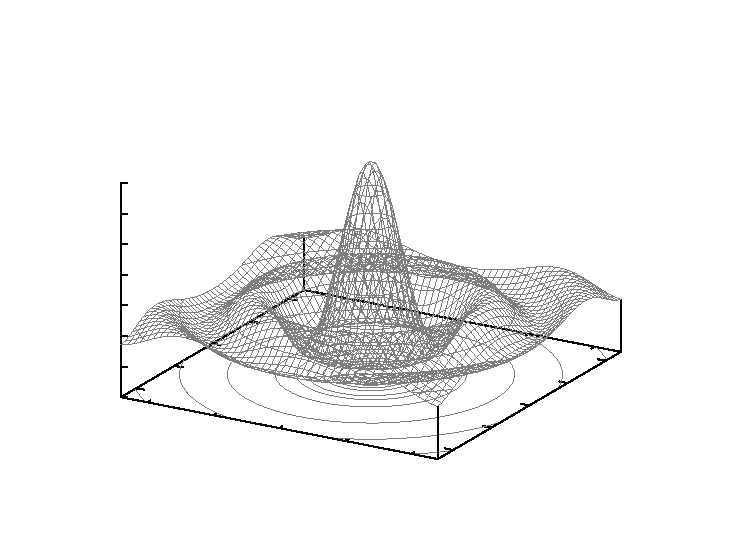
\includegraphics{sincplain}}%
    \gplfronttext
  \end{picture}%
\endgroup

 \end{center}
 \caption[]{\quad The function $f(x,y) = \frac{\sin \sqrt{x^2 + y^2}}{\sqrt{x^2 + y^2}}$.}
 \label{fig:sinc}
\end{figure}
\end{exmp}
\hrule width \textwidth height 0.5pt
\medskip

You may be wondering what happens to the function in Example \ref{exmp:sinc} at the point $(x,y) = (0,0)$, since both
the numerator and denominator are $0$ at that point. 
The function is not defined at $(0,0)$, but the
\emph{limit} of the function exists (and equals $1$) as $(x,y)$ \emph{approaches} $(0,0)$. 
We will now state explicitly
what is meant by the limit of a function of two variables.

\statedefn{defn:mlim}{\index{limit}
 {Let $(a,b)$ be a point in $\Real{2}$, and let $f(x,y)$ be a real-valued function defined on some set
 containing $(a,b)$ (but not necessarily defined at $(a,b)$ itself). 
 Then we say that the \textbf{limit} of
 $f(x,y)$ equals $L$ as $(x,y)$ approaches $(a,b)$, written as
 \begin{equation}\label{eqn:mlim}
  \lim_{(x,y) \to (a,b)} f(x,y) = L ~,
 \end{equation}
 if given any $\epsilon > 0$, there exists a $\delta > 0$ such that
 \begin{displaymath}
  \abs{f(x,y) - L} < \epsilon \text{~~~whenever~~~} 0 < \sqrt{(x-a)^2 + (y-b)^2} < \delta .
 \end{displaymath}}
}

A similar definition can be made for functions of three variables.
The idea behind the above definition is that the values of $f(x,y)$ can get arbitrarily close to $L$ (i.e. within $\epsilon$ of $L$) 
if we pick $(x,y)$ sufficiently close to $(a,b)$ (i.e. inside a circle centered at
$(a,b)$ with some sufficiently small radius $\delta$).

If you recall the ``epsilon-delta'' proofs of limits of real-valued functions of a single variable, you may remember
how awkward they can be, and how they can usually only be done easily for simple functions. 
In general, the
multivariable cases are at least equally awkward to go through, so we will not bother with such proofs. 
Instead, we
will simply state that when the function $f(x,y)$ is given by a single formula and is defined at the point
$(a,b)$ (e.g. is not some indeterminate form like $0/0$) then you can just substitute $(x,y) = (a,b)$ into the formula
for $f(x,y)$ to find the limit.

\medskip
\hrule width \textwidth height 0.5pt
\begin{exmp}
 \begin{displaymath}
 \lim_{(x,y) \to (1,2)}~ \frac{xy}{x^2 + y^2} = \frac{(1)(2)}{1^2 + 2^2} = \frac{2}{5}
 \end{displaymath}
 since $f(x,y) = \frac{xy}{x^2 + y^2}$ is properly defined at the point $(1,2)$.
\end{exmp}
\hrule width \textwidth height 0.5pt
\medskip

The major difference between limits in one variable and limits in two or more variables has to do with how a point is
approached. 
In the single-variable case, the statement ``$x \rightarrow a$'' means that $x$ gets closer to the value $a$
from two possible directions along the real number line (see
Figure \ref{fig:mlim}(a)). 
In two dimensions, however, $(x,y)$ can approach a point $(a,b)$ along an infinite
number of paths (see Figure \ref{fig:mlim}(b)).

\begin{figure}[h]
 \centering
 \subfloat[][$x \rightarrow a$ in $\mathbb{R}$]{\includegraphics{fig2.1.2a.0}}
 \qquad
 \subfloat[][$(x,y) \rightarrow (a,b)$ in $\Real{2}$]{\includegraphics{fig2.1.2b.0}}
 \caption[]{\quad ``Approaching'' a point in different dimensions.}
 \label{fig:mlim}
\end{figure}

\begin{exmp}
 \begin{displaymath}
 \lim_{(x,y) \to (0,0)}~ \frac{xy}{x^2 + y^2} \text{~~~does not exist}
 \end{displaymath}
 Note that we can not simply substitute $(x,y) = (0,0)$ into the function, since doing so gives an indeterminate
 form $0/0$. 
 To show that the limit does not exist, we will show that the function approaches different values as
 $(x,y)$ approaches $(0,0)$ along different paths in $\Real{2}$.
 To see this, suppose that $(x,y) \rightarrow (0,0)$ along the positive $x$-axis, so that $y = 0$ along that path. 
 Then
 \begin{displaymath}
  f(x,y) = \frac{xy}{x^2 + y^2} = \frac{x 0}{x^2 + 0^2} = 0
 \end{displaymath}
 along that path (since $x > 0$ in the denominator). 
 But if
 $(x,y) \rightarrow (0,0)$ along the straight line $y = x$ through the origin, for $x > 0$, then we see that
 \begin{displaymath}
  f(x,y) = \frac{xy}{x^2 + y^2} = \frac{x^2}{x^2 + x^2} = \frac{1}{2},
 \end{displaymath}
 which means that $f(x,y)$ approaches different values as $(x,y) \rightarrow (0,0)$ along different paths. 
 Hence the
 limit does not exist.
\end{exmp}
\hrule width \textwidth height 0.5pt
\medskip

Limits of real-valued multivariable functions obey the same algebraic rules as in the single-variable case, as shown
in the following theorem, which we state without proof.
\statethm{thm:mlimalg}{
 {Suppose that $\displaystyle\lim_{(x,y) \to (a,b)} f(x,y)$ and $\displaystyle\lim_{(x,y) \to (a,b)} g(x,y)$ both
 exist, and that $k$ is some scalar. 
 Then:
 \begin{enumerate}[(a)]
  \item $\displaystyle\lim_{(x,y) \to (a,b)} \lbrack f(x,y) \pm g(x,y) \rbrack =
   \biggl[ ~\displaystyle\lim_{(x,y) \to (a,b)} f(x,y) ~\biggr] \pm \biggl[ ~\displaystyle\lim_{(x,y) \to (a,b)} g(x,y)
   ~\biggr]$;
  \item $\displaystyle\lim_{(x,y) \to (a,b)} k\,f(x,y) =
   k \, \biggl[ ~\displaystyle\lim_{(x,y) \to (a,b)} f(x,y) ~\biggr]$;
  \item $\displaystyle\lim_{(x,y) \to (a,b)} \lbrack f(x,y) g(x,y) \rbrack =
   \biggl[ ~\displaystyle\lim_{(x,y) \to (a,b)} f(x,y) ~\biggr] \biggl[ ~\displaystyle\lim_{(x,y) \to (a,b)} g(x,y)
   ~\biggr]$;
  \item $\displaystyle\lim_{(x,y) \to (a,b)} \dfrac{f(x,y)}{g(x,y)} =
   \dfrac{\displaystyle\lim_{(x,y) \to (a,b)} f(x,y)}{\displaystyle\lim_{(x,y) \to (a,b)} g(x,y)}~~$ if
   $\displaystyle\lim_{(x,y) \to (a,b)} g(x,y) \ne 0$;
  \item If $\abs{f(x,y) - L} \le g(x,y)$ for all $(x,y)$ and if $\displaystyle\lim_{(x,y) \to (a,b)} g(x,y) = 0$, then
  $\displaystyle\lim_{(x,y) \to (a,b)} f(x,y) = L$.
 \end{enumerate}
 }
}

Note that in part (e), it suffices to have $\abs{f(x,y) - L} \le g(x,y)$ for all $(x,y)$ ``sufficiently
close'' to $(a,b)$ (but excluding $(a,b)$ itself).

\begin{exmp}\label{exmp:discont}
 Show that
 \begin{displaymath}
  \lim_{(x,y) \to (0,0)}~ \frac{y^4}{x^2 + y^2} = 0.
 \end{displaymath}
 Since substituting $(x,y) = (0,0)$ into the function gives the indeterminate form $0/0$, we need an alternate
 method for evaluating this limit. 
 We will use Theorem \ref{thm:mlimalg}(e). 
 First, notice that
 $y^4 = \bigl( \sqrt{y^2} \bigr)^4$ and so $0 \le y^4 \le \bigl( \sqrt{x^2 + y^2} \bigr)^4$ for all $(x,y)$. 
 But $\bigl( \sqrt{x^2 + y^2} \bigr)^4 = (x^2 + y^2)^2$. 
 Thus, for all $(x,y) \ne (0,0)$ we have
 \begin{displaymath}
  \left| \frac{y^4}{x^2 + y^2} \right| \le \frac{(x^2 + y^2)^2}{x^2 + y^2} = x^2 + y^2 \rightarrow 0 \text{~~as~~}
  (x,y) \rightarrow (0,0).
 \end{displaymath}
 Therefore $\displaystyle\lim_{(x,y) \to (0,0)} \frac{y^4}{x^2 + y^2} = 0$.
\end{exmp}
\hrule width \textwidth height 0.5pt
\medskip

Continuity can be defined similarly as in the single-variable case.

\statedefn{defn:mcont}{\index{function!continuous}\index{continuity}
 {A real-valued function $f(x,y)$ with domain $D$ in $\Real{2}$ is \textbf{continuous} at the
 point $(a,b)$ in $D$ if $\displaystyle\lim_{(x,y) \to (a,b)} f(x,y) = f(a,b)$. We say that $f(x,y)$ is a
 \textbf{continuous function} if it is continuous at every point in its domain $D$.}
}

Unless indicated otherwise, you can assume that all the functions we deal with are continuous. 
In fact, we can
modify the function from Example \ref{exmp:discont} so that it is continuous on all of $\Real{2}$.

\medskip
\hrule width \textwidth height 0.5pt
\begin{exmp}
 Define a function $f(x,y)$ on all of $\Real{2}$ as follows:
 \begin{displaymath}
  f(x,y) =
  \begin{cases}
   0 & \text{if $(x,y) = (0,0)$}\\
   \dfrac{y^4}{x^2 + y^2} & \text{if $(x,y) \ne (0,0)$}
  \end{cases}
 \end{displaymath}
 Then $f(x,y)$ is well-defined for all $(x,y)$ in $\Real{2}$ (i.e. there are no indeterminate forms for any
 $(x,y)$), and we see that
 \begin{displaymath}
  \lim_{(x,y) \to (a,b)} f(x,y) = \frac{b^4}{a^2 + b^2} = f(a,b) \text{~~~for $(a,b) \ne (0,0)$.}
 \end{displaymath}
 So since 
 \begin{displaymath}
  \lim_{(x,y) \to (0,0)} f(x,y) = 0 = f(0,0) \text{~~~by Example \ref{exmp:discont},}
 \end{displaymath}
 then $f(x,y)$ is continuous on all of $\Real{2}$.
\end{exmp}
\hrule width \textwidth height 0.5pt

%\startexercises
\centerline{\fbox{\textsf{\textbf{\large Exercises}}}}\label{sec2dot1}
\probs{A}
\par\noindent For Exercises 1--6, state the domain and range of the given function.
\begin{enumerate}[\bfseries 1.]
 \begin{multicols}{2}
  \item $f(x,y) = x^2 + y^2 - 1; \phantom{\dfrac{1}{x^2}}$
  \item $f(x,y) = \dfrac{1}{x^2 + y^2}$;
 \end{multicols}
 \begin{multicols}{2}
  \item $f(x,y) = \sqrt{x^2 + y^2 - 4}; \phantom{\dfrac{x^2}{y}}$
  \item $f(x,y) = \dfrac{x^2 + 1}{y}$;
 \end{multicols}
 \begin{multicols}{2}
  \item $f(x,y,z) = \sin (xyz)$;
  \item $f(x,y,z) = \sqrt{(x-1)(yz-1)}$.
 \end{multicols}
\suspend{enumerate}
\par\noindent For Exercises 7--18, evaluate the given limit.
\resume{enumerate}[{[\bfseries 1.]}]
 \begin{multicols}{2}
  \item $\displaystyle\lim_{(x,y) \to (0,0)}~ \cos (xy)$;
  \item $\displaystyle\lim_{(x,y) \to (0,0)}~ e^{xy}$;
 \end{multicols}
 \begin{multicols}{2}
  \item $\displaystyle\lim_{(x,y) \to (0,0)}~ \dfrac{x^2 - y^2}{x^2 + y^2}$;
  \item $\displaystyle\lim_{(x,y) \to (0,0)}~ \dfrac{xy^2}{x^2 + y^4}$;
 \end{multicols}
 \begin{multicols}{2}
  \item $\displaystyle\lim_{(x,y) \to (1,-1)}~ \dfrac{x^2 - 2xy + y^2}{x - y}$;
  \item $\displaystyle\lim_{(x,y) \to (0,0)}~ \dfrac{xy^2}{x^2 + y^2}$;
 \end{multicols}
 \begin{multicols}{2}
  \item $\displaystyle\lim_{(x,y) \to (1,1)}~ \dfrac{x^2 - y^2}{x - y}$;
  \item $\displaystyle\lim_{(x,y) \to (0,0)}~ \dfrac{x^2 - 2xy + y^2}{x - y}$;
 \end{multicols}
 \begin{multicols}{2}
  \item $\displaystyle\lim_{(x,y) \to (0,0)}~ \dfrac{y^4 \sin (xy)}{x^2 + y^2}$;
  \item $\displaystyle\lim_{(x,y) \to (0,0)}~ (x^2 + y^2) \cos \left( \frac{1}{xy} \right)$;
 \end{multicols}
 \begin{multicols}{2}
  \item $\displaystyle\lim_{(x,y) \to (0,0)}~ \dfrac{x}{y}$;
  \item $\displaystyle\lim_{(x,y) \to (0,0)}~ \cos \left( \frac{1}{xy} \right)$.
 \end{multicols}
\suspend{enumerate}
\probs{B}
\resume{enumerate}[{[\bfseries 1.]}]
 \item Show that $f(x,y)= \frac{1}{2\pi\sigma^2}e^{-(x^2 + y^2 )/2\sigma^2}$, for $\sigma >0$, is constant on the circle
  of radius $r > 0$ centered at the origin. 
  This function is called a \emph{Gaussian blur}\index{Gaussian blur}, and is
  used as a filter in image processing software to produce a ``blurred'' effect.
 \item Suppose that $f(x,y) \le f(y,x)$ for all $(x,y)$ in $\Real{2}$. 
 Show that $f(x,y) = f(y,x)$ for all
  $(x,y)$ in $\Real{2}$.
 \item Use the substitution $r=\sqrt{x^2 + y^2}$ to show that
  \begin{displaymath}
   \displaystyle\lim_{(x,y) \to (0,0)}~ \dfrac{\sin \sqrt{x^2 + y^2}}{\sqrt{x^2 + y^2}} = 1 ~.
  \end{displaymath}
  (\emph{Hint: You will need to use L'H{\^o}pital's Rule for single-variable limits.})
\suspend{enumerate}
\probs{C}
\resume{enumerate}[{[\bfseries 1.]}]
 \item Prove Theorem \ref{thm:mlimalg}(a) in the case of addition. 
 (\emph{Hint: Use Definition \ref{defn:mlim}.})
 \item Prove Theorem \ref{thm:mlimalg}(b).
\end{enumerate}
\newpage
%Begin Section 2.2
\section{Partial Derivatives}
Now that we have an idea of what functions of several variables are, and what a limit of such a function is, we can
start to develop an idea of a derivative of a function of two or more variables. 
We will start with the notion of a
\emph{partial derivative}.
\index{partial derivative}
\index{derivative!partial}
\index{$\dfrac{\partial f}{\partial x}$}

\statedefn{defn:partial}{\index{$\partial$}
 {Let $f(x,y)$ be a real-valued function with domain $D$ in $\Real{2}$, and let $(a,b)$ be a point in $D$. 
 Then the \textbf{partial derivative of $\bm{f}$ at $\bm{(a,b)}$ with respect to $\bm{x}$}, denoted by
  $\dfrac{\partial f}{\partial x} (a,b)$, is defined as
  \begin{equation}\label{eqn:parx}
   \dfrac{\partial f}{\partial x} (a,b) = \lim_{h \to 0} \dfrac{f(a+h,b) - f(a,b)}{h}
  \end{equation}
  and the \textbf{partial derivative of $\bm{f}$ at $\bm{(a,b)}$ with respect to $\bm{y}$}, denoted by
  $\dfrac{\partial f}{\partial y} (a,b)$, is defined as
  \begin{equation}\label{eqn:pary}
   \dfrac{\partial f}{\partial y} (a,b) = \lim_{h \to 0} \dfrac{f(a,b+h) - f(a,b)}{h} ~.
  \end{equation}
  Note: The symbol $\partial$ is pronounced ``del''.\footnotemark}
}\footnotetext{It is not a Greek letter. 
The symbol was first used by the mathematicians A. Clairaut and L. Euler
around 1740, to distinguish it from the letter $d$ used for the ``usual'' derivative.}

Recall that the derivative of a function $f(x)$ can be interpreted as the rate of change of that function in the
(positive) $x$ direction. 
From the definitions above, we can see that the partial derivative of a function $f(x,y)$ with respect to $x$ or $y$ is the rate of change of $f(x,y)$ in the (positive) $x$ or $y$ direction,
respectively. 
What this means is that the partial derivative of a function $f(x,y)$ with respect to $x$ can be
calculated by treating the $y$ \emph{variable} as a \emph{constant}, and then simply differentiating $f(x,y)$ as if it
were a function of $x$ alone, using the usual rules from single-variable calculus. 
Likewise, the partial derivative of
$f(x,y)$ with respect to $y$ is obtained by treating the $x$ variable as a constant and then differentiating $f(x,y)$
as if it were a function of $y$ alone.

\medskip
\hrule width \textwidth height 0.5pt
\begin{exmp}
 Find $\dfrac{\partial f}{\partial x} (x,y)$ and $\dfrac{\partial f}{\partial y} (x,y)$ for the function
 $f(x,y) = x^{2}y + y^3$.\smallskip
 \par\noindent\emph{Solution:} Treating $y$ as a constant and differentiating $f(x,y)$ with respect to $x$ gives
 \begin{displaymath}
  \dfrac{\partial f}{\partial x} (x,y) = 2xy
 \end{displaymath}
 and treating $x$ as a constant and differentiating $f(x,y)$ with respect to $y$ gives
 \begin{displaymath}
  \dfrac{\partial f}{\partial y} (x,y) = x^2 + 3y^2 ~.
 \end{displaymath}
\end{exmp}
\hrule width \textwidth height 0.5pt

We will often simply write $\dfrac{\partial f}{\partial x}$ and $\dfrac{\partial f}{\partial y}$ instead of
$\dfrac{\partial f}{\partial x} (x,y)$ and $\dfrac{\partial f}{\partial y} (x,y)$.

\medskip
\hrule width \textwidth height 0.5pt
\begin{exmp}
 Find $\dfrac{\partial f}{\partial x}$ and $\dfrac{\partial f}{\partial y}$ for the function
 $f(x,y) = \dfrac{\sin (xy^2)}{x^2 + 1}$.\smallskip
 \par\noindent\emph{Solution:} Treating $y$ as a constant and differentiating $f(x,y)$ with respect to $x$ gives
 \begin{displaymath}
  \dfrac{\partial f}{\partial x} = \dfrac{(x^2 + 1)(y^2 \cos (xy^2)) - (2x)\,\sin (xy^2)}{(x^2 + 1)^2}
 \end{displaymath}
 and treating $x$ as a constant and differentiating $f(x,y)$ with respect to $y$ gives
 \begin{displaymath}
  \dfrac{\partial f}{\partial y} = \dfrac{2xy\,\cos (xy^2)}{x^2 + 1} ~.
 \end{displaymath}
\end{exmp}
\hrule width \textwidth height 0.5pt
\medskip

Since both $\dfrac{\partial f}{\partial x}$ and $\dfrac{\partial f}{\partial y}$ are themselves functions of $x$ and
$y$, we can take \emph{their} partial derivatives with respect to $x$ and $y$. 
This yields the \emph{higher-order partial derivatives}:
\begin{gather*}
 \dfrac{\partial^2 f}{\partial x^2} = \dfrac{\partial}{\partial x} \biggl( \dfrac{\partial f}{\partial x} \biggr),
 \qquad
 \dfrac{\partial^2 f}{\partial y^2} =\dfrac{\partial}{\partial y} \biggl( \dfrac{\partial f}{\partial y} \biggr),
 \\
 \dfrac{\partial^2 f}{\partial y \, \partial x} = \dfrac{\partial}{\partial y} \biggl( \dfrac{\partial f}{\partial x}
  \biggr),
  \qquad
 \dfrac{\partial^2 f}{\partial x \, \partial y} = \dfrac{\partial}{\partial x} \biggl( \dfrac{\partial f}{\partial y}
  \biggr),
  \\
 \dfrac{\partial^3 f}{\partial x^3} = \dfrac{\partial}{\partial x} \biggl( \dfrac{\partial^2 f}{\partial x^2} \biggr),
 \qquad
 \dfrac{\partial^3 f}{\partial y^3} =\dfrac{\partial}{\partial y} \biggl( \dfrac{\partial^2 f}{\partial y^2}
 \biggr),
 \\
 \dfrac{\partial^3 f}{\partial y \, \partial x^2} =
  \dfrac{\partial}{\partial y} \biggl( \dfrac{\partial^2 f}{\partial x^2} \biggr),
  \qquad
 \dfrac{\partial^3 f}{\partial x \, \partial y^2} =
  \dfrac{\partial}{\partial x} \biggl( \dfrac{\partial^2 f}{\partial y^2} \biggr),
  \\
 \dfrac{\partial^3 f}{\partial y^2 \, \partial x} =
  \dfrac{\partial}{\partial y} \biggl( \dfrac{\partial^2 f}{\partial y \, \partial x} \biggr),
  \qquad
 \dfrac{\partial^3 f}{\partial x^2 \, \partial y} =
  \dfrac{\partial}{\partial x} \biggl( \dfrac{\partial^2 f}{\partial x \, \partial y} \biggr),
  \\
 \dfrac{\partial^3 f}{\partial x \, \partial y \, \partial x} =
  \dfrac{\partial}{\partial x} \biggl( \dfrac{\partial^2 f}{\partial y \, \partial x} \biggr),
  \qquad
 \dfrac{\partial^3 f}{\partial y \, \partial x \, \partial y} =
  \dfrac{\partial}{\partial y} \biggl( \dfrac{\partial^2 f}{\partial x \, \partial y} \biggr),
  \\
 \vdots
\end{gather*}

\medskip
\hrule width \textwidth height 0.5pt
\begin{exmp}
 Find the partial derivatives $\dfrac{\partial f}{\partial x}$, $\dfrac{\partial f}{\partial y}$,
 $\dfrac{\partial^2 f}{\partial x^2}$,
 $\dfrac{\partial^2 f}{\partial y^2}$, $\dfrac{\partial^2 f}{\partial y \, \partial x}$ and
 $\dfrac{\partial^2 f}{\partial x \, \partial y}$ for the function
 $f(x,y) = e^{x^2 y} + xy^3$.\smallskip
 \par\noindent\emph{Solution:} Proceeding as before, we have
 \begin{alignat*}{2}
  \dfrac{\partial f}{\partial x} &= 2xy e^{x^2 y} + y^3,
  \qquad\qquad
  & \dfrac{\partial f}{\partial y} &= x^2 e^{x^2 y} + 3xy^2,
  \\
  \dfrac{\partial^2 f}{\partial x^2} &= \dfrac{\partial}{\partial x} (2xy e^{x^2 y} + y^3)\qquad\qquad
  & \dfrac{\partial^2 f}{\partial y^2} &= \dfrac{\partial}{\partial y} (x^2 e^{x^2 y} + 3xy^2)
  \\
  \phantom{\dfrac{\partial^2 f}{\partial x^2}} &= 2y e^{x^2 y} + 4x^2 y^2 e^{x^2 y},
  \qquad\qquad
   & \phantom{\dfrac{\partial^2 f}{\partial y^2}} &= x^4 e^{x^2 y} + 6xy,
   \\
  \dfrac{\partial^2 f}{\partial y \, \partial x} &= \dfrac{\partial}{\partial y} (2xy e^{x^2 y} + y^3)
  \qquad\qquad
  & \dfrac{\partial^2 f}{\partial x \, \partial y} &= \dfrac{\partial}{\partial x} (x^2 e^{x^2 y} + 3xy^2)
  \\
  \phantom{\dfrac{\partial^2 f}{\partial y \, \partial x}} &= 2x e^{x^2 y} + 2x^3 y e^{x^2 y} + 3y^2,
  \qquad\qquad
   & \phantom{\dfrac{\partial^2 f}{\partial x \, \partial y}} &= 2x e^{x^2 y} + 2x^3 y e^{x^2 y} + 3y^2.
 \end{alignat*}
\end{exmp}
\hrule width \textwidth height 0.5pt
\medskip

Higher-order partial derivatives that are taken with respect to different variables, such as
$\frac{\partial^2 f}{\partial y \, \partial x}$ and $\frac{\partial^2 f}{\partial x \, \partial y}$, are called
\textbf{mixed partial derivatives}.\index{mixed partial derivative}\index{derivative!mixed partial}
Notice in the above example that $\frac{\partial^2 f}{\partial y \, \partial x} =
\frac{\partial^2 f}{\partial x \, \partial y}$. 
It turns that this will usually be the case. 
Specifically,
whenever both $\frac{\partial^2 f}{\partial y \, \partial x}$ and $\frac{\partial^2 f}{\partial x \, \partial y}$ are
continuous at a point $(a,b)$, then they are equal at that point.\footnote{See pp. 214--216
in \cite{tm} for a proof.} All the functions we will deal with will have continuous partial derivatives of all
orders, so you can assume in the remainder of the text that
\begin{displaymath}
 \frac{\partial^2 f}{\partial y \, \partial x} = \frac{\partial^2 f}{\partial x \, \partial y} ~~
 \text{for all $(x,y)$ in the domain of $f$.}
\end{displaymath}
In other words, it doesn't matter
in which order you take partial derivatives. 
This applies even to mixed partial derivatives of order $3$ or higher.

The notation for partial derivatives varies. 
All of the following are equivalent:
\begin{gather*}
 \dfrac{\partial f}{\partial x}:~ \ssub{f}{x}(x,y) ~, \quad \ssub{f}{1}(x,y) ~, \quad \ssub{D}{x}(x,y) ~, \quad
  \ssub{D}{1}(x,y)~;
  \\
 \dfrac{\partial f}{\partial y}:~ \ssub{f}{y}(x,y) ~, \quad \ssub{f}{2}(x,y) ~, \quad \ssub{D}{y}(x,y) ~, \quad
  \ssub{D}{2}(x,y)~;
  \\
 \dfrac{\partial^2 f}{\partial x^2}:~ \ssub{f}{xx}(x,y) ~, \quad \ssub{f}{11}(x,y) ~, \quad \ssub{D}{xx}(x,y) ~, \quad
  \ssub{D}{11}(x,y)~;
  \\
 \dfrac{\partial^2 f}{\partial y^2}:~ \ssub{f}{yy}(x,y) ~, \quad \ssub{f}{22}(x,y) ~, \quad \ssub{D}{yy}(x,y) ~, \quad
  \ssub{D}{22}(x,y)~;
  \\
 \dfrac{\partial^2 f}{\partial y \, \partial x}: ~ \ssub{f}{xy}(x,y) ~, \quad \ssub{f}{12}(x,y) ~, \quad
  \ssub{D}{xy}(x,y) ~, \quad
  \ssub{D}{12}(x,y)~;
  \\
 \dfrac{\partial^2 f}{\partial x \, \partial y}: ~ \ssub{f}{yx}(x,y) ~, \quad \ssub{f}{21}(x,y) ~, \quad
  \ssub{D}{yx}(x,y) ~, \quad
  \ssub{D}{21}(x,y)~.
\end{gather*}
%\startexercises
\centerline{\fbox{\textsf{\textbf{\large Exercises}}}}\label{sec2dot2}
\probs{A}
\par\noindent For Exercises 1--16, find $\frac{\partial f}{\partial x}$ and $\frac{\partial f}{\partial y}$.
\begin{enumerate}[\bfseries 1.]
 \begin{multicols}{2}
  \item $f(x,y) = x^2 + y^2$;
  \item $f(x,y) = \cos(x+y)$;
 \end{multicols}
 \begin{multicols}{2}
  \item $f(x,y) = \sqrt{x^2 + y + 4}$;
  \item $f(x,y) = \dfrac{x + 1}{y + 1}$;
 \end{multicols}
 \begin{multicols}{2}
  \item $f(x,y) = e^{xy} + xy$;
  \item $f(x,y) = x^2 - y^2 + 6xy + 4x - 8y + 2$;
 \end{multicols}
 \begin{multicols}{2}
  \item $f(x,y) = x^4$;
  \item $f(x,y) = x + 2y$;
 \end{multicols}
 \begin{multicols}{2}
  \item $f(x,y) = \sqrt{x^2 + y^2}$;
  \item $f(x,y) = \sin(x+y)$;
 \end{multicols}
 \begin{multicols}{2}
  \item $f(x,y) = \sqrt[3]{x^2 + y + 4}$;
  \item $f(x,y) = \dfrac{xy + 1}{x + y}$;
 \end{multicols}
 \begin{multicols}{2}
  \item $f(x,y) = e^{-(x^2 + y^2)}$;
  \item $f(x,y) = \ln (xy)$;
 \end{multicols}
 \begin{multicols}{2}
  \item $f(x,y) = \sin(xy)$;
  \item $f(x,y) = \tan(x+y)$.
 \end{multicols}
\suspend{enumerate}
\par\noindent For Exercises 17--26, find $\frac{\partial^2 f}{\partial x^2}$, $\frac{\partial^2 f}{\partial y^2}$
and $\frac{\partial^2 f}{\partial y \, \partial x}$ (use Exercises 1--8, 14, 15).
\resume{enumerate}[{[\bfseries 1.]}]
 \begin{multicols}{2}
  \item $f(x,y) = x^2 + y^2$;
  \item $f(x,y) = \cos(x+y)$;
 \end{multicols}
 \begin{multicols}{2}
  \item $f(x,y) = \sqrt{x^2 + y + 4}$;
  \item $f(x,y) = \dfrac{x + 1}{y + 1}$;
 \end{multicols}
 \begin{multicols}{2}
  \item $f(x,y) = e^{xy} + xy$;
  \item $f(x,y) = x^2 - y^2 + 6xy + 4x - 8y + 2$;
 \end{multicols}
 \begin{multicols}{2}
  \item $f(x,y) = x^4$;
  \item $f(x,y) = x + 2y$;
 \end{multicols}
 \begin{multicols}{2}
  \item $f(x,y) = \ln (xy)$;
  \item $f(x,y) = \sin(xy)$.
 \end{multicols}
\suspend{enumerate}
\probs{B}
\resume{enumerate}[{[\bfseries 1.]}]
 \item Show that the function $f(x,y)=\sin(x+y) + \cos(x-y)$ satisfies the \emph{wave equation}\index{wave
 equation}
  \begin{displaymath}
   \frac{\partial^2 f}{\partial x^2} - \frac{\partial^2 f}{\partial y^2} = 0 ~.
  \end{displaymath}
  The wave equation is an example of a \emph{partial differential equation}.\index{partial differential equation}
 \item Let $u$ and $v$ be twice-differentiable functions of a single variable, and let $c\ne 0$ be a constant.
  Show that $f(x,y)=u(x+cy)+v(x-cy)$ is a
  solution of the \emph{general one-dimensional wave equation}\footnote{Conversely, it turns out that \emph{any}
  solution must be of this form. See Ch. 1 in \cite{wei}.}
  \begin{displaymath}
   \frac{\partial^2 f}{\partial x^2} - \frac{1}{c^2}\,\frac{\partial^2 f}{\partial y^2} = 0 ~.
  \end{displaymath}
\end{enumerate}
\newpage
%Begin Section 2.3
\section{Tangent Plane to a Surface}
In the previous section we mentioned that the partial derivatives $\frac{\partial f}{\partial x}$ and
$\frac{\partial f}{\partial y}$ can be thought of as the rate of change of a function $z = f(x,y)$ in the positive
$x$ and $y$ directions, respectively. Recall that the derivative $\frac{dy}{dx}$ of a function $y = f(x)$
has a geometric meaning, namely as the slope of the tangent line to the graph of $f$ at the point $(x,f(x))$ in
$\Real{2}$. There is a similar geometric meaning to the partial derivatives $\frac{\partial f}{\partial x}$ and
$\frac{\partial f}{\partial y}$ of a function $z = f(x,y)$: given a point $(a,b)$ in the domain $D$ of
$f(x,y)$, the trace of the
surface described by $z = f(x,y)$ in the plane $y = b$ is a curve in $\Real{3}$ through the point $(a,b,f(a,b))$, and
the slope of the tangent line $L_x$ to that curve at that point is $\frac{\partial f}{\partial x}(a,b)$. Similarly,
$\frac{\partial f}{\partial y}(a,b)$ is the slope of the tangent line $L_y$ to the trace of the surface $z = f(x,y)$ in
the plane $x = a$ (see Figure \ref{fig:partial}).\index{tangent plane}\index{plane!tangent}

\begin{figure}[h]
 \centering
 \subfloat[][Tangent line $L_x$ in the plane $y = b$]{
 \begin{tikzpicture}
  \usetikzlibrary{arrows}
  \definecolor{planecolor}{HTML}{FFB270}
  \fill [opacity=0.5,blue!60] (2.53,1.92) to[out=220,in=80] (1.75,0.95) -- (1.75,-1.4) -- (2.53,-0.62) -- (2.53,1.92);
  \shade [opacity=0.1,ball color=red!40] [rotate around={-20:(2.0,1.5)}] (2.0,1.5) ellipse (1.58 and 0.6);
  \draw [black!60,line width=0.3pt] (0,0) -- (1.75,0,0);
  \draw [dashed,black!60,line width=0.3pt] (1.75,0) -- (2.53,0,0);
  \draw [black!60,line width=0.3pt,-latex] (2.53,0) -- (4,0,0);
  \draw [black!60,line width=0.3pt,-latex] (0,0) -- (0,3,0);
  \draw [black!60,line width=0.3pt,-latex] (0,0) -- (0,0,4);
  \pgfputat{\pgfpointxyz{3.9}{0.2}{0}}{\pgfbox[center,center]{\small $y$}};
  \pgfputat{\pgfpointxyz{0.2}{2.9}{0}}{\pgfbox[center,center]{\small $z$}};
  \pgfputat{\pgfpointxyz{0.2}{0}{3.8}}{\pgfbox[center,center]{\small $x$}};
  \pgfputat{\pgfpointxyz{0.05}{-0.2}{0}}{\pgfbox[center,center]{\small $0$}};
  \draw [dashed,line width=0.2pt] (0.5,-1) arc (180:360:1.5 and 0.4);
  \draw [dashed,line width=0.2pt] (3.5,-1) arc (0:180:1.5 and 0.4);
  \draw [rotate around={-20:(2.0,1.5)}] (2.0,1.5) ellipse (1.58 and 0.6);
  \fill (2.3,-0.85) circle (1pt);
  \fill (2.3,1.75) circle (1.2pt);
  \node [below] at (2.5,-0.85) {\small $(a,b)$};
  \node [below] at (2.0,-1.4) {\small $D$};
  \draw [black!60,line width=0.1pt] (3.15,0) -- (1.75,-1.4);
  \draw [line width=0.2pt] (2.53,1.92) to[out=220,in=80] (1.75,0.95);
  \draw [line width=0.2pt] (2.7,2.05) -- (1.25,0.9);
  \node [left,below] at (1.25,0.9) {\small $L_x$};
  \node [above] at (3.15,0) {\small $b$};
  \node [left] at (2.35,1.85) {\small $(a,b,f(a,b))$};
  \node [right] at (2.8,2) {\small slope $= \tfrac{\partial f}{\partial x}(a,b)$};
  \node [right] at (0.5,2.6) {\small $z = f(x,y)$};
 \end{tikzpicture}}
 \qquad\qquad
 \subfloat[][Tangent line $L_y$ in the plane $x = a$]{
 \begin{tikzpicture}
  \usetikzlibrary{arrows}
  \definecolor{planecolor}{HTML}{FFB270}
  \definecolor{surfcolor}{HTML}{006146}
  \fill [opacity=0.5,blue!60] (0.65,2.2) to[out=-20,in=110] (3.35,0.8) -- (3.35,-0.85) -- (0.65,-0.85) -- (0.65,2.2);
  \shade [opacity=0.1,ball color=red!40] [rotate around={-20:(2.0,1.5)}] (2.0,1.5) ellipse (1.58 and 0.6);
  \draw [black!60,line width=0.3pt] (0,0) -- (0.65,0,0);
  \draw [dashed,black!60,line width=0.3pt] (0.65,0) -- (3.35,0,0);
  \draw [black!60,line width=0.3pt,-latex] (3.35,0) -- (4,0,0);
  \draw [black!60,line width=0.3pt,-latex] (0,0) -- (0,3,0);
  \draw [black!60,line width=0.3pt,-latex] (0,0) -- (0,0,4);
  \pgfputat{\pgfpointxyz{3.9}{0.2}{0}}{\pgfbox[center,center]{\small $y$}};
  \pgfputat{\pgfpointxyz{0.2}{2.9}{0}}{\pgfbox[center,center]{\small $z$}};
  \pgfputat{\pgfpointxyz{0.2}{0}{3.8}}{\pgfbox[center,center]{\small $x$}};
  \pgfputat{\pgfpointxyz{0.05}{-0.2}{0}}{\pgfbox[center,center]{\small $0$}};
  \draw [dashed,line width=0.2pt] (0.5,-1) arc (180:360:1.5 and 0.4);
  \draw [dashed,line width=0.2pt] (3.5,-1) arc (0:180:1.5 and 0.4);
  \draw [rotate around={-20:(2.0,1.5)}] (2.0,1.5) ellipse (1.58 and 0.6);
  \fill (2.3,-0.85) circle (1pt);
  \fill (2.3,1.75) circle (1.2pt);
  \node [below] at (2.3,-0.85) {\small $(a,b)$};
  \node [below] at (2.0,-1.4) {\small $D$};
  \draw [black!60,line width=0.1pt] (-0.85,-0.85) -- (0.5,-0.85);
  \draw [black!60,line width=0.1pt] (0.65,-0.85) -- (3.35,-0.85);
  \draw [line width=0.2pt] (0.65,2.2) to[out=-20,in=110] (3.35,0.8);
  \draw [line width=0.2pt] (0.5,2.5) -- (4,1.07);
  \node [right,below] at (4,1.07) {\small $L_y$};
  \node [left] at (-0.85,-0.85) {\small $a$};
  \node [left] at (2.6,1.5) {\small $(a,b,f(a,b))$};
  \node [right] at (0.5,2.6) {\small slope $= \tfrac{\partial f}{\partial y}(a,b)$};
  \node [right] at (2.8,2) {\small $z = f(x,y)$};
 \end{tikzpicture}}
 \caption[]{\quad Partial derivatives as slopes.}
 \label{fig:partial}
\end{figure}

Since the derivative $\tfrac{dy}{dx}$ of a function $y = f(x)$ is used to find the tangent line to the graph of
$f$ (which is a curve in $\Real{2}$), you might expect that partial derivatives can be used to define a
\emph{tangent plane} to the graph of a surface $z = f(x,y)$. This indeed turns out to be the case. First, we need a
definition of a tangent plane. The intuitive idea is that a tangent plane ``just touches'' a surface at a point.
The formal definition mimics the intuitive notion of a tangent line to a curve.

\statedefn{defn:tanplane}{
 {Let $z = f(x,y)$ be the equation of a surface $S$ in $\Real{3}$, and let $P = (a,b,c)$ be a point on $S$.
  Let $T$ be a plane which contains the point $P$, and let $Q = (x,y,z)$ represent a generic point on the surface $S$.
  If the (acute) angle between the vector $\overrightarrow{PQ}$ and the plane $T$ approaches zero as the point $Q$
  approaches $P$ along the surface $S$, then we call $T$ the \textbf{tangent plane} to $S$ at $P$.}
}

Note that since two lines in $\Real{3}$ determine a plane, then the two tangent lines to the surface $z=f(x,y)$ in the
$x$ and $y$ directions described in Figure \ref{fig:partial} are contained in the tangent plane at that point, \emph{if
the tangent plane exists at that point}.
The existence of those two tangent lines does not by itself guarantee the
existence of the tangent plane. It is possible that if we take the trace of the surface in the plane $x-y=0$ (which
makes a $45\Degrees$ angle with the positive $x$-axis), the resulting curve in that plane may have a tangent line
which is not in the plane determined by the other two tangent lines, or it may not have a tangent line at all at that
point. Luckily, it turns out\footnote{See \cite[\S\,6.4]{tm}.} that if $\frac{\partial f}{\partial x}$ and
$\frac{\partial f}{\partial y}$ exist in a region around a point $(a,b)$ and are continuous at $(a,b)$ then the
tangent plane to the surface $z=f(x,y)$ will exist at the point $(a,b,f(a,b))$. In this text, those conditions will
always hold.

\piccaption[]{\quad Tangent plane}\parpic[r]{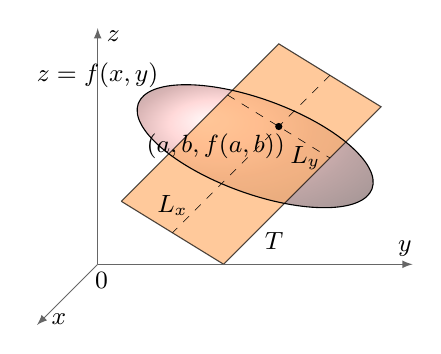
\begin{tikzpicture}
  \usetikzlibrary{arrows}
  \definecolor{planecolor}{HTML}{FFB270}
  \shade [opacity=0.5,ball color=red!40] [rotate around={-20:(2.0,1.5)}] (2.0,1.5) ellipse (1.58 and 0.6);
  \filldraw [opacity=0.7,black,fill=planecolor] (0.3,0.8) -- (1.6,0) -- (3.6,2) -- (2.3,2.8) -- (0.3,0.8);
  \draw [black!60,line width=0.3pt,-latex] (0,0) -- (4,0,0);
  \draw [black!60,line width=0.3pt,-latex] (0,0) -- (0,3,0);
  \draw [black!60,line width=0.3pt,-latex] (0,0) -- (0,0,2);
  \pgfputat{\pgfpointxyz{3.9}{0.2}{0}}{\pgfbox[center,center]{\small $y$}};
  \pgfputat{\pgfpointxyz{0.2}{2.9}{0}}{\pgfbox[center,center]{\small $z$}};
  \pgfputat{\pgfpointxyz{0.2}{0}{1.8}}{\pgfbox[center,center]{\small $x$}};
  \pgfputat{\pgfpointxyz{0.05}{-0.2}{0}}{\pgfbox[center,center]{\small $0$}};
  \draw [rotate around={-20:(2.0,1.5)}] (2.0,1.5) ellipse (1.58 and 0.6);
  \fill (2.3,1.75) circle (1.3pt);
  \draw [line width=0.2pt,dashed] (2.95,2.4) -- (0.95,0.4);
  \draw [line width=0.2pt,dashed] (1.65,2.15) -- (2.95,1.35);
  \node [left] at (2.5,1.5) {\small $(a,b,f(a,b))$};
  \node at (0,2.4) {\small $z = f(x,y)$};
  \node [right] at (2,0.3) {\small $T$};
  \node [above] at (0.95,0.5) {\small $L_x$};
  \node [left] at (2.95,1.35) {\small $L_y$};
 \end{tikzpicture}}
Suppose that we want an equation of the tangent plane $T$ to the surface $z=f(x,y)$ at a point $(a,b,f(a,b))$.
Let $\ssub{L}{x}$ and $\ssub{L}{y}$ be the tangent lines to the traces of the surface in the planes $y=b$ and $x=a$,
respectively (as in Figure 2.3.2), and suppose that the conditions for $T$ to exist do hold. Then the
equation for $T$ is
\begin{equation}
 A(x-a)+B(y-b)+C(z-f(a,b))=0
\end{equation}
where $\textbf{n}=(A,B,C)$ is a normal vector to the plane $T$. Since $T$ contains the lines $\ssub{L}{x}$ and
$\ssub{L}{y}$, then all we need are vectors $\ssub{\textbf{v}}{x}$ and $\ssub{\textbf{v}}{y}$ that are parallel to
$\ssub{L}{x}$ and
$\ssub{L}{y}$, respectively, and then let $\textbf{n}=\Crossprod{\ssub{\textbf{v}}{x}}{\ssub{\textbf{v}}{y}}$.

\piccaption[]{}\parpic[r]{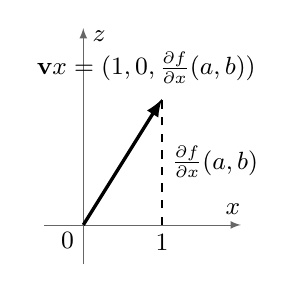
\begin{tikzpicture}
   \usetikzlibrary{arrows}
   \draw [black!60,line width=0.3pt,-latex] (-0.5,0) -- (2,0);
   \draw [black!60,line width=0.3pt,-latex] (0,-0.5) -- (0,2.5);
   \pgfputat{\pgfpointxyz{1.9}{0.2}{0}}{\pgfbox[center,center]{\small $x$}}
   \pgfputat{\pgfpointxyz{0.2}{2.4}{0}}{\pgfbox[center,center]{\small $z$}}
   \pgfputat{\pgfpointxyz{-0.2}{-0.2}{0}}{\pgfbox[center,center]{\small $0$}}
   \draw [black,line width=1.2,-latex] (0,0) -- (1,1.6);
   \node at (0.8,2) {\small $\ssub{\textbf{v}}{x}=(1,0,\frac{\partial f}{\partial x}(a,b))$};
   \node [right] at (1,0.8) {\small $\frac{\partial f}{\partial x}(a,b)$};
   \node [below] at (1,0) {\small $1$};
   \draw [dashed] (1,0) -- (1,1.6);
  \end{tikzpicture}}
\par\noindent Since the slope of
$\ssub{L}{x}$ is $\frac{\partial f}{\partial x}(a,b)$, then the vector
$\ssub{\textbf{v}}{x}=(1,0,\frac{\partial f}{\partial x}(a,b))$ is parallel to $\ssub{L}{x}$ (since
$\ssub{\textbf{v}}{x}$ lies in the
$xz$-plane and lies in a line with slope $\frac{\frac{\partial f}{\partial x}(a,b)}{1}=
\frac{\partial f}{\partial x}(a,b)$. See Figure 2.3.3).
Similarly, the vector\\$\ssub{\textbf{v}}{y}=(0,1,\frac{\partial f}{\partial y}(a,b))$ is parallel to $\ssub{L}{y}$.
Hence, the vector
\begin{displaymath}
 \textbf{n} = \Crossprod{\ssub{\textbf{v}}{x}}{\ssub{\textbf{v}}{y}} =
  \left|
  \begin{array}{rrr}
   \textbf{i} & \textbf{j} & \textbf{k}\\
   1 & 0 & \tfrac{\partial f}{\partial x}(a,b)\\
   0 & 1 & \tfrac{\partial f}{\partial y}(a,b)
  \end{array}\right|
  = -\tfrac{\partial f}{\partial x}(a,b)\,\textbf{i} - \tfrac{\partial f}{\partial y}(a,b)\,\textbf{j} + \textbf{k}
\end{displaymath}
is normal to the plane $T$. Thus the equation of $T$ is
\begin{equation}
 -\tfrac{\partial f}{\partial x}(a,b)\,(x-a) - \tfrac{\partial f}{\partial y}(a,b)\,(y-b)+z-f(a,b)=0 ~.
\end{equation}
Multiplying both sides by $-1$, we have the following result:\smallskip
\statecomment{
 The equation of the tangent plane to the surface $z=f(x,y)$ at the point $(a,b,f(a,b))$ is
 \begin{equation}\label{eqn:tanplane}
  \tfrac{\partial f}{\partial x}(a,b)\,(x-a) + \tfrac{\partial f}{\partial y}(a,b)\,(y-b)-z+f(a,b)=0
 \end{equation}}

\begin{exmp}
 Find the equation of the tangent plane to the surface $z =  x^2 + y^2$ at the point $(1,2,5)$.\smallskip
 \par\noindent \emph{Solution:} For the function $f(x,y) = x^2 + y^2$, we have
 $\tfrac{\partial f}{\partial x} = 2x$ and $\tfrac{\partial f}{\partial y} = 2y$, so the equation of the tangent plane
 at the point $(1,2,5)$ is
 \begin{gather*}
  2(1)(x-1)+2(2)(y-2)-z+5=0 \text{~,~or}\\
  2x+4y-z-5=0 ~.
 \end{gather*}
\end{exmp}
\hrule width \textwidth height 0.5pt
\medskip

In a similar fashion, it can be shown that if a surface is defined implicitly by an equation of the form
$F(x,y,z)=0$, then the tangent plane to the surface at a point $(a,b,c)$ is given by the equation
\begin{equation}\label{eqn:imptanplane}
 \tfrac{\partial F}{\partial x}(a,b,c)\,(x-a) + \tfrac{\partial F}{\partial y}(a,b,c)\,(y-b) +
 \tfrac{\partial F}{\partial z}(a,b,c)\,(z-c) = 0 ~.
\end{equation}
Note that formula (\ref{eqn:tanplane}) is the special case of formula (\ref{eqn:imptanplane}) where
$F(x,y,z) = f(x,y) - z$.
\medskip
\hrule width \textwidth height 0.5pt
\begin{exmp}
 Find the equation of the tangent plane to the surface $x^2 + y^2 + z^2 = 9$ at the point $(2,2,-1)$.\smallskip
 \par\noindent \emph{Solution:} For the function $F(x,y,z) = x^2 + y^2 + z^2 - 9$, we have
 $\tfrac{\partial F}{\partial x} = 2x$, $\tfrac{\partial F}{\partial y} = 2y$, and
 $\tfrac{\partial F}{\partial z} = 2z$, so the equation of the tangent plane at $(2,2,-1)$ is
 \begin{gather*}
  2(2)(x-2)+2(2)(y-2)+2(-1)(z+1)=0 \text{~,~or}\\
  2x+2y-z-9=0 ~.
 \end{gather*}
\end{exmp}
\startexercises\label{sec2dot3}
\probs{A}
\par\noindent For Exercises 1--6, find the equation of the tangent plane to the surface $z=f(x,y)$ at the point
$P$.
\begin{enumerate}[\bfseries 1.]
 \begin{multicols}{2}
  \item $f(x,y) = x^2 + y^3$, $P=(1,1,2)$;
  \item $f(x,y) = xy$, $P=(1,-1,-1)$;
 \end{multicols}
 \begin{multicols}{2}
  \item $f(x,y) = x^2 y$, $P=(-1,1,1)$;
  \item $f(x,y) = xe^y$, $P=(1,0,1)$;
 \end{multicols}
 \begin{multicols}{2}
  \item $f(x,y) = x+2y$, $P=(2,1,4)$;
  \item $f(x,y) = \sqrt{x^2 + y^2}$, $P=(3,4,5)$.
 \end{multicols}
\suspend{enumerate}
\par\noindent For Exercises 7--10, find the equation of the tangent plane to the given surface at the point $P$.
\resume{enumerate}[{[\bfseries 1.]}]
 \begin{multicols}{2}
  \item $\frac{x^2}{4} + \frac{y^2}{9}  + \frac{z^2}{16} = 1$, $P=\left(1,2,\frac{2\sqrt{11}}{3}\right)$;
  \item $x^2 + y^2 +z^2 = 9$, $P=(0,0,3)$;
 \end{multicols}
 \begin{multicols}{2}
  \item $x^2 + y^2 - z^2 = 0$, $P=(3,4,5)$;
  \item $x^2 + y^2 = 4$, $P=(\sqrt{3},1,0)$.
 \end{multicols}
\end{enumerate}
\newpage
%Begin Section 2.4
\section{Directional Derivatives and the Gradient}
For a function $z=f(x,y)$, we learned that the partial derivatives $\tfrac{\partial f}{\partial x}$ and
$\tfrac{\partial f}{\partial y}$ represent the (instantaneous) rate of change of $f$ in the positive $x$ and $y$
directions, respectively. What about other directions? It turns out that we can find the rate of change in
\emph{any} direction using a more general type of derivative called a \emph{directional derivative}.

\statedefn{defn:dirderiv}{\index{directional derivative}\index{derivative!directional}
 {Let $f(x,y)$ be a real-valued function with domain $D$ in $\Real{2}$, and let $(a,b)$ be a point in $D$. Let
  \textbf{v} be a vector in $\Real{2}$. Then the
  \textbf{directional derivative of $\bm{f}$ at $\bm{(a,b)}$ in the direction of v}, denoted by
  $\ssub{D}{\textbf{v}}f(a,b)$, is defined as
  \begin{equation}\label{eqn:dirderiv}
   \ssub{D}{\textbf{v}}f(a,b) = \lim_{h \to 0} \dfrac{f((a,b) + h\textbf{v}) - f(a,b)}{h}.
  \end{equation}}
}

Notice in the definition that we seem to be treating the point $(a,b)$ as a vector, since we are adding the
vector $h\textbf{v}$ to it. But this is just the usual idea of identifying vectors with their terminal points, which
the reader should be used to by now. If we were to write the vector \textbf{v} as $\textbf{v} = \vectwo{v}$, then
\begin{equation}\label{eqn:dirderivpt}
 \ssub{D}{\textbf{v}}f(a,b) = \lim_{h \to 0} \dfrac{f(a+h\ssub{v}{1},b+h\ssub{v}{2}) - f(a,b)}{h} ~.
\end{equation}
From this we can immediately recognize that the partial derivatives $\tfrac{\partial f}{\partial x}$ and
$\tfrac{\partial f}{\partial y}$ are special cases of the directional derivative with $\textbf{v} = \textbf{i} = (1,0)$
and $\textbf{v} = \textbf{j} = (0,1)$, respectively. 
That is, $\tfrac{\partial f}{\partial x} = \ssub{D}{\textbf{i}}f$
and $\tfrac{\partial f}{\partial y} = \ssub{D}{\textbf{j}}f$. 

If $f(x,y)$ has continuous partial derivatives $\tfrac{\partial f}{\partial x}$ and
$\tfrac{\partial f}{\partial y}$ (which will always be the case in this text), then there is a simple formula for the
directional derivative:\index{$\ssub{D}{\textbf{v}}f$}

\statethm{thm:dirderiv}{
 {Let $f(x,y)$ be a real-valued function with domain $D$ in $\Real{2}$ such that the partial derivatives
 $\tfrac{\partial f}{\partial x}$ and $\tfrac{\partial f}{\partial y}$ exist and are continuous in $D$. Let $(a,b)$ be
 a point in $D$. Then
  \begin{equation}\label{eqn:dirderivfor}
   \ssub{D}{\textbf{v}}f(a,b) = \ssub{v}{1}\frac{\partial f}{\partial x}(a,b) +
    \ssub{v}{2}\frac{\partial f}{\partial y}(a,b) ~.
  \end{equation}}
  for any vector $\textbf{v} = \vectwo{v}$ in $\Real{2}$
}
\begin{proofbar}
\begin{proof}[Proof:]
 Note that if $\textbf{v} = \textbf{i} = (1,0)$ then the above formula reduces to
 $\ssub{D}{\textbf{v}}f(a,b) = \tfrac{\partial f}{\partial x}(a,b)$, which we know is true since
 $\ssub{D}{\textbf{i}}f = \tfrac{\partial f}{\partial x}$, as we noted earlier. Similarly, for
 $\textbf{v} = \textbf{j} = (0,1)$ the formula reduces to $\ssub{D}{\textbf{v}}f(a,b) =
 \tfrac{\partial f}{\partial y}(a,b)$, which is true since $\ssub{D}{\textbf{j}}f = \tfrac{\partial f}{\partial y}$.
 Fix such a vector $\textbf{v} = \vectwo{v}$ and fix a number $h \ne 0$.
Then
 \begin{equation}\label{eqn:dirderivdiff}
  f(a+h\ssub{v}{1},b+h\ssub{v}{2}) - f(a,b) = f(a+h\ssub{v}{1},b+h\ssub{v}{2}) - f(a+h\ssub{v}{1},b) +
   f(a+h\ssub{v}{1},b) - f(a,b) ~.
 \end{equation}
 Since $g(\alpha)=f(a+h\ssub{v}{1},y+\alpha h\ssub{v}{2})$ is a real-valued function,
 we can apply
 the Mean Value Theorem from single-variable calculus on the interval $[0,1]$.
 It provides a number $0 < \alpha < 1$ such that
 \begin{align*}
  g\,'(\alpha) 
  &= 
   \frac{g(1) - g(0)}{1-0} 
   \\
   &=
   f(a+h\ssub{v}{1},b+h\ssub{v}{2}) - f(a+h\ssub{v}{1},b).
 \end{align*}
 By chain rule
 \[g\,'(\alpha)=\frac{\partial f}{\partial y}(a+h\ssub{v}{1},b+\alpha h\ssub{v}{2}) h\ssub{v}{2}.\]
 Therefore 
 \[f(a+h\ssub{v}{1},b+h\ssub{v}{2}) - f(a+h\ssub{v}{1},b)
 =
 h\ssub{v}{2}\frac{\partial f}{\partial x}(a+h\ssub{v}{1},b+\alpha h\ssub{v}{2}) .\]
 By a similar argument, there exists a number $0 < \beta < 1$ such that
 \begin{displaymath}
  f(a+h\ssub{v}{1},b) - f(a,b) = h\ssub{v}{1} \frac{\partial f}{\partial x}(a+\beta h\ssub{v}{1},b) ~.
 \end{displaymath}
 Thus, by equation (\ref{eqn:dirderivdiff}), we have
 \begin{align*}
  \frac{f(a+h\ssub{v}{1},b+h\ssub{v}{2}) - f(a,b)}{h} ~~ &= ~~
   \frac{h\ssub{v}{2}\tfrac{\partial f}{\partial y}(a+h\ssub{v}{1},b+\alpha h\ssub{v}{2}) +
    h\ssub{v}{1} \tfrac{\partial f}{\partial x}(a+\beta h\ssub{v}{1},b)}{h}\\[6pt]
   &= ~~ \ssub{v}{2}\frac{\partial f}{\partial y}(a+h\ssub{v}{1},b+\alpha h\ssub{v}{2}) +
    \ssub{v}{1} \frac{\partial f}{\partial x}(a+\beta h\ssub{v}{1},b)
 \end{align*}
 so by formula (\ref{eqn:dirderivpt}) we have
 \begin{align*}
  \ssub{D}{\textbf{v}}f(a,b) ~~ &= ~~ \lim_{h \to 0} \dfrac{f(a+h\ssub{v}{1},b+h\ssub{v}{2}) - f(a,b)}{h}\\[8pt]
   &= ~~ \lim_{h \to 0} \left[ \ssub{v}{2}\frac{\partial f}{\partial y}(a+h\ssub{v}{1},b+\alpha h\ssub{v}{2}) +
    \ssub{v}{1} \frac{\partial f}{\partial x}(a+\beta h\ssub{v}{1},b) \right]\\[8pt]
   &= ~~ \ssub{v}{2}\frac{\partial f}{\partial y}(a,b) +
    \ssub{v}{1}\frac{\partial f}{\partial x}(a,b) \text{~~~by the continuity of $\frac{\partial f}{\partial x}$ and
     $\frac{\partial f}{\partial y}$, so}\\[8pt]
   \ssub{D}{\textbf{v}}f(a,b) ~~ &= ~~ \ssub{v}{1}\frac{\partial f}{\partial x}(a,b) +
    \ssub{v}{2}\frac{\partial f}{\partial y}(a,b)
 \end{align*}
 after reversing the order of summation.
\end{proof}\end{proofbar}

Note that $\ssub{D}{\textbf{v}}f(a,b) = \Dotprod{\textbf{v}}{\biggl(\frac{\partial f}{\partial x}(a,b),
\frac{\partial f}{\partial y}(a,b)\biggr)}$. The second vector has a special name:

\statedefn{defn:grad}{\index{gradient}
 {For a real-valued function $f(x,y)$, the \textbf{gradient} of $f$, denoted by $\nabla f$, is the vector
  \begin{equation}\label{eqn:gradxy}
   \nabla f = \biggl(\frac{\partial f}{\partial x},\frac{\partial f}{\partial y}\biggr)
  \end{equation}
  in $\Real{2}$. 
  For a real-valued function $f(x,y,z)$, the gradient is the vector
  \begin{equation}\label{eqn:gradxyz}
   \nabla f = \biggl(\frac{\partial f}{\partial x},\frac{\partial f}{\partial y},\frac{\partial f}{\partial z}\biggr)
  \end{equation}
  in $\Real{3}$. The symbol $\nabla$ is pronounced ``del'' or ``nabla''.\footnotemark}
}\footnotetext{Sometimes the notation grad($f$) is used instead of $\nabla f$.}


\statecor{cor:dirderiv}{
 {$\ssub{D}{\textbf{v}}f = \Dotprod{\textbf{v}}{\nabla f}$}
}

\hrule width \textwidth height 0.5pt
\begin{exmp}
 Find the directional derivative of $f(x,y) = xy^2 + x^3 y$ at the point $(1,2)$ in the direction of
 $\textbf{v} = \biggl( \frac{1}{\sqrt{2}},\frac{1}{\sqrt{2}} \biggr)$.\smallskip
 \par\noindent\emph{Solution:} We see that $\nabla f = (y^2 + 3x^2 y, 2xy + x^3)$, so\index{$\nabla$}
 \begin{displaymath}
  \ssub{D}{\textbf{v}}f(1,2) ~=~ \Dotprod{\textbf{v}}{\nabla f(1,2)}
   ~=~ \Dotprod{\biggl( \tfrac{1}{\sqrt{2}},\tfrac{1}{\sqrt{2}} \biggr)}{(2^2 + 3(1)^2 (2),2(1)(2)+1^3)}
   ~=~ \tfrac{15}{\sqrt{2}}
 \end{displaymath}
\end{exmp}
\hrule width \textwidth height 0.5pt
\medskip

A real-valued function $z=f(x,y)$ whose partial derivatives $\tfrac{\partial f}{\partial x}$ and
$\frac{\partial f}{\partial y}$ exist and are continuous is called \emph{continuously differentiable}.
Assume that $f(x,y)$ is such a function and that $\nabla f \ne \textbf{0}$. 
Let $c$ be a real number in the range of
$f$ and let \textbf{v} be a vector in $\Real{2}$ which is tangent to the
level curve $f(x,y) = c$ (see Figure \ref{fig:gradlevel}).
\index{continuously differentiable}
\begin{figure}[h]
 \begin{center}
  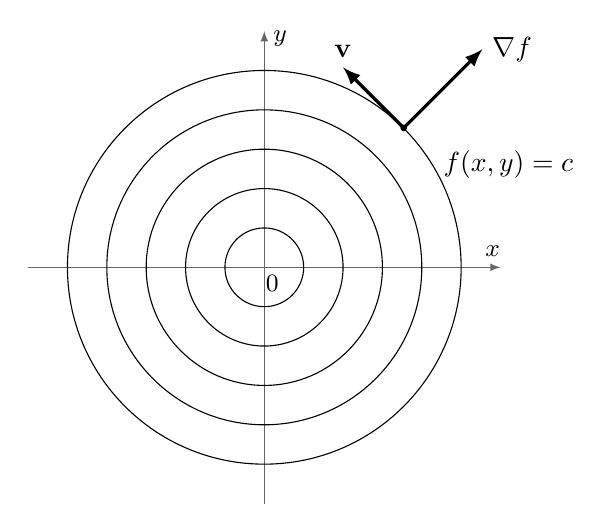
\begin{tikzpicture}
   \usetikzlibrary{arrows}
   \draw [black!60,line width=0.3pt,-latex] (-3,0) -- (3,0);
   \draw [black!60,line width=0.3pt,-latex] (0,-3) -- (0,3);
   \pgfputat{\pgfpointxyz{2.9}{0.2}{0}}{\pgfbox[center,center]{\small $x$}}
   \pgfputat{\pgfpointxyz{0.2}{2.9}{0}}{\pgfbox[center,center]{\small $y$}}
   \pgfputat{\pgfpointxyz{0.1}{-0.2}{0}}{\pgfbox[center,center]{\small $0$}}
   \draw (0,0) circle (0.5);
   \draw (0,0) circle (1);
   \draw (0,0) circle (1.5);
   \draw (0,0) circle (2);
   \draw (0,0) circle (2.5);
   \fill (1.77,1.77) circle (1.2pt);
   \draw [black,line width=1.2pt,-latex] (1.77,1.77) -- (1,2.54);
   \node [above] at (1,2.54) {\textbf{v}};
   \draw [black,line width=1.2pt,-latex] (1.77,1.77) -- (2.77,2.77);
   \node [right] at (2.77,2.77) {$\nabla f$};
   \node at (3.1,1.3) {$f(x,y) = c$};
  \end{tikzpicture}
 \end{center}
 \caption[]{}
 \label{fig:gradlevel}
\end{figure}

The value of $f(x,y)$ is constant along a level curve, so since \textbf{v} is a tangent vector to this curve, then
the rate of change of $f$ in the direction of \textbf{v} is 0, i.e. $\ssub{D}{\textbf{v}}f = 0$. 
But we know that
$\ssub{D}{\textbf{v}}f = \Dotprod{\textbf{v}}{\nabla f}$.
In other words, $\nabla f
\perp \textbf{v}$, which means that $\nabla f$ is \emph{normal} to the level curve.\index{normal to a curve}

In general, for any unit vector \textbf{v} in $\Real{2}$, we have 
$\ssub{D}{\textbf{v}}f = \norm{\nabla f}\,\cos \theta$, where $\theta$ is the angle between \textbf{v} and $\nabla f$.
At a fixed point $(x,y)$ the length $\norm{\nabla f}$ is fixed,
and the value of $\ssub{D}{\textbf{v}}f$ then varies as $\theta$ varies. The largest value
that $\ssub{D}{\textbf{v}}f$ can take is when $\cos \theta = 1$ ($\theta = 0\Degrees$), while the smallest value occurs
when $\cos \theta = -1$ ($\theta = 180\Degrees$). In other words, the value of the function $f$ increases the fastest
in the direction of $\nabla f$ (since $\theta = 0\Degrees$ in that case), and the value of $f$ decreases the fastest in
the direction of $-\nabla f$ (since $\theta = 180\Degrees$ in that case). We have thus proved the following theorem:

\statethm{thm:gradprop}{
 {Let $f(x,y)$ be a continuously differentiable real-valued function, with $\nabla f \ne \textbf{0}$. Then:
 \begin{enumerate}[(a)]
  \item The gradient $\nabla f$ is normal to any level curve $f(x,y)=c$.
  \item The value of $f(x,y)$ increases the fastest in the direction of $\nabla f$.
  \item The value of $f(x,y)$ decreases the fastest in the direction of $-\nabla f$.
 \end{enumerate}}
}

\medskip
\hrule width \textwidth height 0.5pt
\begin{exmp}
 In which direction does the function $f(x,y) = xy^2 + x^3 y$ increase the fastest from the point $(1,2)$?
 In which direction does it decrease the fastest?\smallskip
 \par\noindent\emph{Solution:} Since $\nabla f = (y^2 + 3x^2 y, 2xy + x^3)$, then
 $\nabla f(1,2) = (10,5) \ne \textbf{0}$. 
 A unit vector in that direction is $\textbf{v} =
 \frac{\nabla f}{\norm{\nabla f}} = \biggl( \frac{2}{\sqrt{5}}, \frac{1}{\sqrt{5}} \biggr)$. 
 Thus, $f$ increases the
 fastest in the direction of $\biggl( \frac{2}{\sqrt{5}}, \frac{1}{\sqrt{5}} \biggr)$ and decreases the fastest in
 the direction of $\biggl( \frac{-2}{\sqrt{5}}, \frac{-1}{\sqrt{5}} \biggr)$.
\end{exmp}
\hrule width \textwidth height 0.5pt
\medskip

Though we proved Theorem \ref{thm:gradprop} for functions of two variables, a similar argument can be used to show
that it also applies to functions of three or more variables. Likewise, the directional derivative in the
three-dimensional case can also be defined by the formula $\ssub{D}{\textbf{v}}f =
\Dotprod{\textbf{v}}{\nabla f}$.

\medskip
\hrule width \textwidth height 0.5pt
\begin{exmp}
 The temperature $T$ of a solid is given by the function 
 \[T(x,y,z) = e^{-x} + e^{-2y} + e^{4z},\] 
 where
 $x$, $y$, $z$ are space coordinates relative to the center of the solid. In which direction from the point $(1,1,1)$
 will the temperature decrease the fastest?\smallskip
 \par\noindent\emph{Solution:} Since $\nabla f = (-e^{-x},-2e^{-2y},4e^{4z})$, then the temperature will decrease the
 fastest in the direction of
 $-\nabla f(1,1,1) = (e^{-1},2e^{-2},-4e^4 )$.
\end{exmp}
\hrule width \textwidth height 0.5pt

%\startexercises
\centerline{\fbox{\textsf{\textbf{\large Exercises}}}}\label{sec2dot4}
\probs{A}
\par\noindent For Exercises 1--10, compute the gradient $\nabla f$.
\begin{enumerate}[\bfseries 1.]
 \begin{multicols}{2}
  \item $f(x,y) = x^2 + y^2 - 1; \phantom{\dfrac{1}{x^2}}$
  \item $f(x,y) = \dfrac{1}{x^2 + y^2}$;
 \end{multicols}
 \begin{multicols}{2}
  \item $f(x,y) = \sqrt{x^2 + y^2 + 4}$;
  \item $f(x,y) = x^2 e^y$;
 \end{multicols}
 \begin{multicols}{2}
  \item $f(x,y) = \ln(xy)$;
  \item $f(x,y) = 2x+5y$;
 \end{multicols}
 \begin{multicols}{2}
  \item $f(x,y,z) = \sin (xyz)$;
  \item $f(x,y,z) = x^2 e^{yz}$;
 \end{multicols}
 \begin{multicols}{2}
  \item $f(x,y,z) = x^2 + y^2 + z^2$;
  \item $f(x,y,z) = \sqrt{x^2 + y^2 + z^2}$.
 \end{multicols}
 \suspend{enumerate}
 \par\noindent For Exercises 11--14, find the directional derivative of $f$ at the point $P$ in the direction of
 $\textbf{v} = \biggl( \frac{1}{\sqrt{2}},\frac{1}{\sqrt{2}} \biggr)$.
 \resume{enumerate}[{[\bfseries 1.]}]
 \begin{multicols}{2}
  \item $f(x,y) = x^2 + y^2 - 1$, $P=(1,1); \phantom{\dfrac{1}{x^2}}$
  \item $f(x,y) = \dfrac{1}{x^2 + y^2}$, $P=(1,1)$;
 \end{multicols}
 \begin{multicols}{2}
  \item $f(x,y) = \sqrt{x^2 + y^2 + 4}$, $P=(1,1)$;
  \item $f(x,y) = x^2 e^y$, $P=(1,1)$.
 \end{multicols}
 \suspend{enumerate}
 \par\noindent For Exercises 15--16, find the directional derivative of $f$ at the point $P$ in the direction of
 $\textbf{v} = \biggl( \frac{1}{\sqrt{3}},\frac{1}{\sqrt{3}},\frac{1}{\sqrt{3}} \biggr)$.
 \resume{enumerate}[{[\bfseries 1.]}]
 \begin{multicols}{2}
  \item $f(x,y,z) = \sin (xyz)$, $P=(1,1,1)$;
  \item $f(x,y,z) = x^2 e^{yz}$, $P=(1,1,1)$.
 \end{multicols}
  \item Repeat Example 2.16 at the point $(2,3)$.
  \item Repeat Example 2.17 at the point $(3,1,2)$.
 \suspend{enumerate}
\probs{B}
\par\noindent For Exercises 19--26, let $f(x,y)$ and $g(x,y)$ be continuously differentiable
real-valued functions, let $c$ be a constant, and let \textbf{v} be a unit vector in $\Real{2}$. Show that:
\resume{enumerate}[{[\bfseries 1.]}]
 \begin{multicols}{2}
  \item $\nabla (cf) = c\,\nabla f$;
  \item $\nabla (f+g) = \nabla f + \nabla g$;
 \end{multicols}
 \begin{multicols}{2}
  \item $\nabla (fg) = f\,\nabla g + g\,\nabla f; \phantom{\dfrac{g\,\nabla f - f\,\nabla g}{g^2}}$
  \item $\nabla (f/g) = \dfrac{g\,\nabla f - f\,\nabla g}{g^2} ~$ if $g(x,y) \ne 0$;
 \end{multicols}
 \begin{multicols}{2}
  \item $\ssub{D}{-\textbf{v}}f = -\ssub{D}{\textbf{v}}f$;
  \item $\ssub{D}{\textbf{v}}(cf) = c\,\ssub{D}{\textbf{v}}f$;
 \end{multicols}
 \begin{multicols}{2}
  \item $\ssub{D}{\textbf{v}}(f+g) = \ssub{D}{\textbf{v}}f ~+~ \ssub{D}{\textbf{v}}g$;
  \item $\ssub{D}{\textbf{v}}(fg) = f\,\ssub{D}{\textbf{v}}g ~+~ g\,\ssub{D}{\textbf{v}}f$.
 \end{multicols}
 \item The function $r(x,y) = \sqrt{x^2 + y^2}$ is the length of the position vector
  $\textbf{r}=x\,\textbf{i} + y\,\textbf{j}$ for each point $(x,y)$ in $\Real{2}$. Show that
  $\nabla r = \dfrac{1}{r}\,\textbf{r}~$ when $(x,y) \ne (0,0)$, and that $\nabla (r^2 ) = 2\,\textbf{r}$.
\end{enumerate}
\newpage
%Begin Section 2.5
\section{Maxima and Minima}
The gradient can be used to find \emph{extreme points} of real-valued functions of several variables, that is,
points where the function has a \emph{local maximum} or \emph{local minimum}. We will consider only functions of two
variables; functions of three or more variables require methods using linear algebra.\index{extreme point}

\statedefn{defn:localext}{\index{local maximum}\index{local minimum}\index{global maximum}\index{global minimum}
 {Let $f(x,y)$ be a real-valued function, and let $(x_0,y_0)$ be a point in the domain of $f$. We say that $f$ has a
  \textbf{local maximum} at $(x_0,y_0)$ if $f(x,y) \le f(x_0,y_0)$ for all $(x,y)$ inside some disk of positive radius centered
  at $(x_0,y_0)$, i.e. there is some sufficiently small $r > 0$ such that $f(x,y) \le f(x_0,y_0)$ for all $(x,y)$ for
  which $(x-x_0)^2 + (y-y_0)^2 < r^2$.
  
  Likewise, we say that $f$ has a \textbf{local minimum} at $(x_0,y_0)$ if $f(x,y) \ge f(x_0,y_0)$ for all $(x,y)$ inside some
  disk of positive radius centered at $(x_0,y_0)$.
  
  If $f(x,y) \le f(x_0,y_0)$ for all $(x,y)$ in the domain of $f$, then $f$ has a \textbf{global maximum} at $(x_0,y_0)$. If
  $f(x,y) \ge f(x_0,y_0)$ for all $(x,y)$ in the domain of $f$, then $f$ has a \textbf{global minimum} at $(x_0,y_0)$.}
}

Suppose that $(x_0,y_0)$ is a local maximum point for $f(x,y)$, and that the first-order partial derivatives of $f$
exist at $(x_0,y_0)$. 
We know that $f(x_0,y_0)$ is the largest value of $f(x,y)$ as $(x,y)$
goes in all directions from the point $(x_0,y_0)$, in some sufficiently small disk centered at $(x_0,y_0)$. 
In particular, $f(x_0,y_0)$ is the largest value of $f$ in the $x$ direction (around the point $(x_0,y_0)$), that is, the
single-variable function $g(x) = f(x,b)$ has a local maximum at $x=a$. So we know that $g\,'(a) = 0$. Since
$g\,'(x) = \frac{\partial f}{\partial x}(x,b)$, then $\frac{\partial f}{\partial x}(x_0,y_0)=0$. 
Similarly, $f(x_0,y_0)$ is the
largest value of $f$ near $(x_0,y_0)$ in the $y$ direction and so $\frac{\partial f}{\partial y}(x_0,y_0)=0$. We thus have the
following theorem:

\statethm{thm:extnec}{
 {Let $f(x,y)$ be a real-valued function such that both $\frac{\partial f}{\partial x}(x_0,y_0)$ and
 $\frac{\partial f}{\partial y}(x_0,y_0)$ exist. 
 Then a necessary condition for $f(x,y)$ to have a local maximum or minimum
 at $(x_0,y_0)$ is that $\nabla f (x_0,y_0) = \textbf{0}$.}
}
Note: Theorem \ref{thm:extnec} can be extended to apply to functions of three or more variables.

A point $(x_0,y_0)$ where $\nabla f (x_0,y_0) = \textbf{0}$ is called a \textbf{critical point} for the function $f(x,y)$.
So given a function $f(x,y)$, to find the critical points of $f$ you have to solve the equations
$\frac{\partial f}{\partial x}(x,y) = 0$ and $\frac{\partial f}{\partial y}(x,y) = 0$ simultaneously for $(x,y)$.
Similar to the single-variable case, the \emph{necessary} condition that $\nabla f (x_0,y_0) = \textbf{0}$ is not always
\emph{sufficient} to guarantee that a critical point is a local maximum or minimum.\index{critical point}

\medskip
\hrule width \textwidth height 0.5pt
\begin{exmp}
 The function $f(x,y) = xy$ has a critical point at $(0,0)$: $\frac{\partial f}{\partial x} = y = 0 \Rightarrow y=0$,
 and $\frac{\partial f}{\partial y} = x = 0 \Rightarrow x=0$, so $(0,0)$ is the only critical point. But clearly $f$
 does not have a local maximum or minimum at $(0,0)$ since any disk around $(0,0)$ contains points $(x,y)$ where the
 values of $x$ and $y$ have the same sign (so that $f(x,y) = xy > 0 = f(0,0)$) and different signs (so that $f(x,y) =
 xy < 0 = f(0,0)$). In fact, along the path $y=x$ in $\Real{2}$, $f(x,y) = x^2$, which has a

\noindent local minimum at $(0,0)$,
 while along the path $y=-x$ we have $f(x,y)=-x^2$, which has a local maximum at $(0,0)$. So $(0,0)$ is an example of a
 \emph{saddle point}, i.e. it is a local maximum in one direction and a local minimum in another direction. The graph
 of $f(x,y)$ is shown in Figure \ref{fig:xy}, which is a hyperbolic paraboloid.\index{paraboloid!hyperbolic}
\end{exmp}
\begin{figure}[h]
 \begin{center}
  % GNUPLOT: LaTeX picture with Postscript
\begingroup
\footnotesize
  \makeatletter
  \providecommand\color[2][]{%
    \GenericError{(gnuplot) \space\space\space\@spaces}{%
      Package color not loaded in conjunction with
      terminal option `colourtext'%
    }{See the gnuplot documentation for explanation.%
    }{Either use 'blacktext' in gnuplot or load the package
      color.sty in LaTeX.}%
    \renewcommand\color[2][]{}%
  }%
  \providecommand\includegraphics[2][]{%
    \GenericError{(gnuplot) \space\space\space\@spaces}{%
      Package graphicx or graphics not loaded%
    }{See the gnuplot documentation for explanation.%
    }{The gnuplot epslatex terminal needs graphicx.sty or graphics.sty.}%
    \renewcommand\includegraphics[2][]{}%
  }%
  \providecommand\rotatebox[2]{#2}%
  \@ifundefined{ifGPcolor}{%
    \newif\ifGPcolor
    \GPcolortrue
  }{}%
  \@ifundefined{ifGPblacktext}{%
    \newif\ifGPblacktext
    \GPblacktexttrue
  }{}%
  % define a \g@addto@macro without @ in the name:
  \let\gplgaddtomacro\g@addto@macro
  % define empty templates for all commands taking text:
  \gdef\gplbacktext{}%
  \gdef\gplfronttext{}%
  \makeatother
  \ifGPblacktext
    % no textcolor at all
    \def\colorrgb#1{}%
    \def\colorgray#1{}%
  \else
    % gray or color?
    \ifGPcolor
      \def\colorrgb#1{\color[rgb]{#1}}%
      \def\colorgray#1{\color[gray]{#1}}%
      \expandafter\def\csname LTw\endcsname{\color{white}}%
      \expandafter\def\csname LTb\endcsname{\color{black}}%
      \expandafter\def\csname LTa\endcsname{\color{black}}%
      \expandafter\def\csname LT0\endcsname{\color[rgb]{1,0,0}}%
      \expandafter\def\csname LT1\endcsname{\color[rgb]{0,1,0}}%
      \expandafter\def\csname LT2\endcsname{\color[rgb]{0,0,1}}%
      \expandafter\def\csname LT3\endcsname{\color[rgb]{1,0,1}}%
      \expandafter\def\csname LT4\endcsname{\color[rgb]{0,1,1}}%
      \expandafter\def\csname LT5\endcsname{\color[rgb]{1,1,0}}%
      \expandafter\def\csname LT6\endcsname{\color[rgb]{0,0,0}}%
      \expandafter\def\csname LT7\endcsname{\color[rgb]{1,0.3,0}}%
      \expandafter\def\csname LT8\endcsname{\color[rgb]{0.5,0.5,0.5}}%
    \else
      % gray
      \def\colorrgb#1{\color{black}}%
      \def\colorgray#1{\color[gray]{#1}}%
      \expandafter\def\csname LTw\endcsname{\color{white}}%
      \expandafter\def\csname LTb\endcsname{\color{black}}%
      \expandafter\def\csname LTa\endcsname{\color{black}}%
      \expandafter\def\csname LT0\endcsname{\color{black}}%
      \expandafter\def\csname LT1\endcsname{\color{black}}%
      \expandafter\def\csname LT2\endcsname{\color{black}}%
      \expandafter\def\csname LT3\endcsname{\color{black}}%
      \expandafter\def\csname LT4\endcsname{\color{black}}%
      \expandafter\def\csname LT5\endcsname{\color{black}}%
      \expandafter\def\csname LT6\endcsname{\color{black}}%
      \expandafter\def\csname LT7\endcsname{\color{black}}%
      \expandafter\def\csname LT8\endcsname{\color{black}}%
    \fi
  \fi
  \setlength{\unitlength}{0.0500bp}%
  \begin{picture}(6802.00,5040.00)%
    \gplgaddtomacro\gplbacktext{%
      \csname LTb\endcsname%
      \put(5969,1567){\makebox(0,0)[l]{\strut{}-10}}%
      \put(5530,1434){\makebox(0,0)[l]{\strut{}-5}}%
      \put(5091,1301){\makebox(0,0)[l]{\strut{} 0}}%
      \put(4652,1168){\makebox(0,0)[l]{\strut{} 5}}%
      \put(4212,1034){\makebox(0,0)[l]{\strut{} 10}}%
      \put(936,1337){\makebox(0,0){\strut{}-10}}%
      \put(1697,1260){\makebox(0,0){\strut{}-5}}%
      \put(2457,1183){\makebox(0,0){\strut{} 0}}%
      \put(3218,1106){\makebox(0,0){\strut{} 5}}%
      \put(3977,1030){\makebox(0,0){\strut{} 10}}%
      \put(876,1370){\makebox(0,0)[r]{\strut{}-100}}%
      \put(876,1944){\makebox(0,0)[r]{\strut{}-50}}%
      \put(876,2518){\makebox(0,0)[r]{\strut{} 0}}%
      \put(876,3091){\makebox(0,0)[r]{\strut{} 50}}%
      \put(876,3664){\makebox(0,0)[r]{\strut{} 100}}%
      \put(563,2385){\makebox(0,0){\strut{}$z$}}%
    }%
    \gplgaddtomacro\gplfronttext{%
      \csname LTb\endcsname%
      \put(5814,1252){\makebox(0,0){\strut{}$x$}}%
      \put(2084,1084){\makebox(0,0){\strut{}$y$}}%
      \put(563,2385){\makebox(0,0){\strut{}$z$}}%
    }%
    \gplbacktext
    \put(0,0){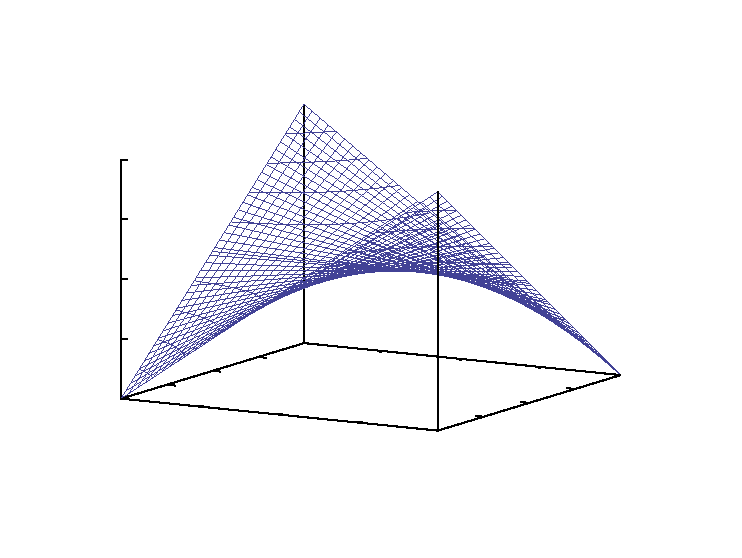
\includegraphics{fig251}}%
    \gplfronttext
  \end{picture}%
\endgroup

 \end{center}
 \caption[]{\quad $f(x,y) = xy$, saddle point at $(0,0)$.}
 \label{fig:xy}
\end{figure}
\hrule width \textwidth height 0.5pt

\medskip

From the course of single-variable calculus, you may remember \emph{second derivative test}.

\statecomment{If $f'(x_0)=0$ and $f''(0)>0$ then the real-to-real function $f$ has a local minimum at $x_0$.}

In order to explain the multi-variable analog of this test,
let us introduce \emph{second directional derivative}. 
Fix a vector $\textbf{v}\in\Real{2}$ and a smooth function of two variables $f(x,y)$.
The directional derivative $h(x,y)=D_{\textbf{v}}f(x,y)$ is an other smooth function of two variables, so we can take its directional derivative again 
$D_{\textbf{v}}h(x,y)$;
it is called \emph{second directional derivative} and denoted as $D_{\textbf{v}}^2f(x,y)$.

\statecomment{If $D_{\textbf{v}}f(x_0,y_0)=0$ and $D_{\textbf{v}}^2f(x_0,y_0)>0$ for any vector $\textbf{v}\ne\textbf{0}$ then the the smooth function $f(x,y)$ of two variables, has a local minimum at $(x_0,y_0)$.}

In this form the second derivative test is not useful
since it requires to check inequality $D_{\textbf{v}}^2f(x_0,y_0)>0$ for infinite number of vectors $\textbf{v}$. 
Let us try to remove this weak point.

Note that 
if $\textbf{v}=(a,b)$ then 
\begin{align*}
D_{\textbf{v}}f(x_0,y_0)&=a\tfrac{\partial f}{\partial x}+b\tfrac{\partial f}{\partial y}.
\intertext{and}
D^2_{\textbf{v}}f(x_0,y_0)&=D_{\textbf{v}}(a\tfrac{\partial f}{\partial x}+b\tfrac{\partial f}{\partial y})
\\
&=a^2\tfrac{\partial^2 f}{\partial x^2}+ab\tfrac{\partial^2 f}{\partial x\partial y}+ab\tfrac{\partial^2 f}{\partial y\partial x}+b^2\tfrac{\partial^2 f}{\partial y^2}
\\
&=a^2\tfrac{\partial^2 f}{\partial x^2}+2ab\tfrac{\partial^2 f}{\partial y\partial x}+b^2\tfrac{\partial^2 f}{\partial y^2},
\end{align*}
the last equality holds since the function $f$ is smooth and therefore $\tfrac{\partial^2 f}{\partial x\partial y}=\tfrac{\partial^2 f}{\partial y\partial x}$


Therefore the condition $D_{\textbf{v}}^2f(x_0,y_0)>0$ for any $\textbf{v}\ne\textbf{0}$
means that 
\[a^2\tfrac{\partial^2 f}{\partial x^2}+2ab\tfrac{\partial^2 f}{\partial y\partial x}+b^2\tfrac{\partial^2 f}{\partial y^2}>0\]
for any pair of real numbers $(a,b)$ at least one of which is not zero.

Analyzing the last inequality for all possible pairs $(a,b)$ leads to the following theorem which is true analog of second derivative test for smooth functions of two variables; it gives sufficient conditions for a critical point to be a local maximum or\index{$D$}
minimum of a \emph{smooth function}\index{smooth function} (i.e. a function whose partial derivatives of all orders
exist and are continuous).
The theorem will not be proved here.\footnote{See \cite[\S\,7.6]{tm}.}\index{Second Derivative Test}

\statethm{thm:extsuff}{
 {Let $f(x,y)$ be a smooth real-valued function, with a critical point at $(x_0,y_0)$ (i.e.
 $\nabla f(x_0,y_0) = \textbf{0}$). Define
 \begin{displaymath}
  D = \dfrac{\partial^2 f}{\partial x^2}(x_0,y_0) \, \dfrac{\partial^2 f}{\partial y^2}(x_0,y_0) -
 \biggl( \dfrac{\partial^2 f}{\partial y \, \partial x}(x_0,y_0) \biggr)^2
 \end{displaymath}
 Then
 \begin{enumerate}[(a)]
  \item if $D > 0$ and $\tfrac{\partial^2 f}{\partial x^2}(x_0,y_0) > 0$, then $f$ has a local minimum at $(x_0,y_0)$
  \item if $D > 0$ and $\tfrac{\partial^2 f}{\partial x^2}(x_0,y_0) < 0$, then $f$ has a local maximum at $(x_0,y_0)$
  \item if $D < 0$, then $f$ has neither a local minimum nor a local maximum at $(x_0,y_0)$
  \item if $D = 0$, then the test fails.
 \end{enumerate}}
}

If condition (c) holds, then $(x_0,y_0)$ is a \emph{saddle point};\index{saddle point}
that is, the second directional derivative 
$D^2_\textbf{v}f(x_0,y_0)$ can be positive and negative for different vectors $\textbf{v}$.

Recall that the assumption that $f(x,y)$ is smooth implies that $\frac{\partial^2 f}{\partial y \, \partial x} = \frac{\partial^2 f}{\partial x \, \partial y}$. Therefore
\begin{displaymath}
 D =
 \begin{vmatrix}
  \dfrac{\partial^2 f}{\partial x^2}(x_0,y_0) & \dfrac{\partial^2 f}{\partial y \, \partial x}(x_0,y_0)\smallskip\\
  \dfrac{\partial^2 f}{\partial x \, \partial y}(x_0,y_0) & \dfrac{\partial^2 f}{\partial y^2}(x_0,y_0)
 \end{vmatrix}.
\end{displaymath} 
Also, if $D > 0$
then $\frac{\partial^2 f}{\partial x^2}(x_0,y_0) \, \frac{\partial^2 f}{\partial y^2}(x_0,y_0) = D +
\biggl( \frac{\partial^2 f}{\partial y \, \partial x}(x_0,y_0) \biggr)^2 > 0$, and so
$\frac{\partial^2 f}{\partial x^2}(x_0,y_0)$ and $\frac{\partial^2 f}{\partial y^2}(x_0,y_0)$ have the same sign. 
This means
that in parts (a) and (b) of the theorem one can replace $\frac{\partial^2 f}{\partial x^2}(x_0,y_0)$ by
$\frac{\partial^2 f}{\partial y^2}(x_0,y_0)$ if desired.

\medskip
\hrule width \textwidth height 0.5pt
\begin{exmp}
 Find all local maxima and minima of $f(x,y) = x^2 + xy + y^2 - 3x$.\smallskip
 \par\noindent\emph{Solution:} First find the critical points, i.e. where $\nabla f = \textbf{0}$. Since
 \begin{displaymath}
  \frac{\partial f}{\partial x} = 2x + y -3 \quad \text{and} \quad \frac{\partial f}{\partial y} = x + 2y
 \end{displaymath}
 then the critical points $(x,y)$ are the common solutions of the equations
 \begin{alignat*}{10}
  2x &+ \phantom{2}y - 3 &&= 0\\
  \phantom{2}x &+ 2y &&= 0
 \end{alignat*}
 which has the unique solution $(x,y) = (2,-1)$. So $(2,-1)$ is the only critical point.
 
 To use Theorem \ref{thm:extsuff}, we need the second-order partial derivatives:
 \begin{displaymath}
  \frac{\partial^2 f}{\partial x^2} = 2 ~,\quad \frac{\partial^2 f}{\partial y^2} = 2 ~,\quad
  \dfrac{\partial^2 f}{\partial y \, \partial x} = 1
 \end{displaymath}
 and so
 \begin{displaymath}
  D ~=~ \dfrac{\partial^2 f}{\partial x^2}(2,-1) \, \dfrac{\partial^2 f}{\partial y^2}(2,-1) -
 \biggl( \dfrac{\partial^2 f}{\partial y \, \partial x}(2,-1) \biggr)^2 ~=~ (2)(2) - 1^2 ~=~ 3 ~>~ 0
 \end{displaymath}
 and $\frac{\partial^2 f}{\partial x^2}(2,-1) = 2 > 0$. Thus, $(2,-1)$ is a local minimum.
 \end{exmp}
\hrule width \textwidth height 0.5pt
\begin{exmp}
 Find all local maxima and minima of $f(x,y) = xy - x^3 - y^2$.\smallskip
 \par\noindent\emph{Solution:} First find the critical points, i.e. where $\nabla f = \textbf{0}$. Since
 \begin{displaymath}
  \frac{\partial f}{\partial x} = y - 3x^2 \quad \text{and} \quad \frac{\partial f}{\partial y} = x - 2y
 \end{displaymath}
then the critical points $(x,y)$ are the common solutions of the equations
 \begin{align*}
  y - 3x^2 &= 0\\
  x - 2y &= 0
 \end{align*}
 The first equation yields $y = 3x^2$, substituting that into the second equation yields $x - 6x^2 = 0$, which
 has the solutions $x = 0$ and $x = \frac{1}{6}$. So $x = 0 \Rightarrow y = 3(0) = 0$ and $x = \frac{1}{6} \Rightarrow
 y = 3\bigl( \frac{1}{6} \bigr)^2 = \frac{1}{12}$.\\
 So the critical points are $(x,y) = (0,0)$ and $(x,y) = \bigl( \frac{1}{6}, \frac{1}{12} \bigr)$.
 
 To use Theorem \ref{thm:extsuff}, we need the second-order partial derivatives:
 \begin{displaymath}
  \frac{\partial^2 f}{\partial x^2} = -6x ~,\quad \frac{\partial^2 f}{\partial y^2} = -2 ~,\quad
  \dfrac{\partial^2 f}{\partial y \, \partial x} = 1
 \end{displaymath}
 So
 \begin{displaymath}
  D ~=~ \dfrac{\partial^2 f}{\partial x^2}(0,0) \, \dfrac{\partial^2 f}{\partial y^2}(0,0) -
 \biggl( \dfrac{\partial^2 f}{\partial y \, \partial x}(0,0) \biggr)^2 ~=~ (-6(0))(-2) - 1^2 ~=~ -1 ~<~ 0
 \end{displaymath}
 and thus $(0,0)$ is a saddle point.
 Also,
 \begin{displaymath}
  D ~=~ \dfrac{\partial^2 f}{\partial x^2}\bigl( \tfrac{1}{6}, \tfrac{1}{12} \bigr) \, 
  \dfrac{\partial^2 f}{\partial y^2}\bigl( \tfrac{1}{6}, \tfrac{1}{12} \bigr) -
 \biggl( \dfrac{\partial^2 f}{\partial y \, \partial x}\bigl( \tfrac{1}{6}, \tfrac{1}{12} \bigr) \biggr)^2 ~=~
 (-6\bigl(\frac{1}{6}\bigr))(-2) - 1^2 ~=~ 1 ~>~ 0
 \end{displaymath}
 and $\frac{\partial^2 f}{\partial x^2}\bigl( \frac{1}{6}, \frac{1}{12} \bigr) = -1 < 0$.
 Thus, $\bigl( \frac{1}{6}, \frac{1}{12} \bigr)$ is a local maximum.
 \end{exmp}
\hrule width \textwidth height 0.5pt
\begin{exmp}\label{exmp:globalmin}
 Find all local maxima and minima of $f(x,y) = (x-2)^4 + (x-2y)^2$.\smallskip
 \par\noindent\emph{Solution:} First find the critical points, i.e. where $\nabla f = \textbf{0}$. Since
 \begin{displaymath}
  \frac{\partial f}{\partial x} = 4(x-2)^3 + 2(x-2y) \quad \text{and} \quad \frac{\partial f}{\partial y} = -4(x-2y)
 \end{displaymath}
 then the critical points $(x,y)$ are the common solutions of the equations
 \begin{align*}
  4(x-2)^3 + 2(x-2y) &= 0\\
  -4(x-2y) &= 0
 \end{align*}
 The second equation yields $x=2y$, substituting that into the first equation yields $4(2y-2)^3 = 0$, which has
 the solution $y=1$, and so $x =2(1) = 2$. Thus, $(2,1)$ is the only critical point.
 
 To use Theorem \ref{thm:extsuff}, we need the second-order partial derivatives:
 \begin{displaymath}
  \frac{\partial^2 f}{\partial x^2} = 12(x-2)^2 + 2 ~,\quad \frac{\partial^2 f}{\partial y^2} = 8 ~,\quad
  \dfrac{\partial^2 f}{\partial y \, \partial x} = -4
 \end{displaymath}
So
 \begin{displaymath}
  D ~=~ \dfrac{\partial^2 f}{\partial x^2}(2,1) \, \dfrac{\partial^2 f}{\partial y^2}(2,1) -
 \biggl( \dfrac{\partial^2 f}{\partial y \, \partial x}(2,1) \biggr)^2 ~=~ (2)(8) - (-4)^2 ~=~ 0
 \end{displaymath}
 and so the test fails. What can be done in this situation? Sometimes it is possible to examine the function to see
 directly the nature of a critical point. In our case, we see that $f(x,y) \ge 0$ for all $(x,y)$, since $f(x,y)$ is
 the sum of fourth and second powers of numbers and hence must be nonnegative. But we also see that $f(2,1) = 0$.
 Thus $f(x,y) \ge 0 = f(2,1)$ for all $(x,y)$, and hence $(2,1)$ is in fact a \emph{global} minimum for $f$.
\end{exmp}
\hrule width \textwidth height 0.5pt
\begin{exmp}
 Find all local maxima and minima of $f(x,y) = (x^2 + y^2 ) e^{-(x^2 + y^2 )}$.\smallskip
 \par\noindent\emph{Solution:} First find the critical points, i.e. where $\nabla f = \textbf{0}$. Since
 \begin{align*}
  \frac{\partial f}{\partial x} ~ &= ~ 2x(1 - (x^2 + y^2 )) e^{-(x^2 + y^2 )}\\[6pt]
  \frac{\partial f}{\partial y} ~ &= ~ 2y(1 - (x^2 + y^2 )) e^{-(x^2 + y^2 )}
 \end{align*}
 then the critical points are $(0,0)$ and all points $(x,y)$ on the unit circle $x^2 + y^2 = 1$.
 
 To use Theorem \ref{thm:extsuff}, we need the second-order partial derivatives:
 \begin{align*}
  \frac{\partial^2 f}{\partial x^2} ~ &= ~2\lbrack 1-(x^2 + y^2 )-2x^2-2x^2(1-(x^2 + y^2 ))\rbrack e^{-(x^2 + y^2 )}\\[6pt]
  \frac{\partial^2 f}{\partial y^2} ~ &= ~ 2\lbrack 1-(x^2 + y^2 )-2y^2-2y^2(1-(x^2 + y^2 ))\rbrack e^{-(x^2 + y^2 )}\\[6pt]
  \dfrac{\partial^2 f}{\partial y \, \partial x} ~ &= ~ -4xy\lbrack 2-(x^2 + y^2 ) \rbrack e^{-(x^2 + y^2 )}
 \end{align*}
 At $(0,0)$, we have $D = 4 > 0$ and $\frac{\partial^2 f}{\partial x^2}(0,0) = 2 > 0$, so $(0,0)$ is a local minimum.
 However, for points $(x,y)$ on the unit circle $x^2 + y^2 = 1$, we have
 \begin{displaymath}
  D ~=~ (-4x^2 e^{-1})(-4y^2 e^{-1}) - (-4xy e^{-1})^2 ~=~ 0
 \end{displaymath}
 and so the test fails. If we look at the graph of $f(x,y)$, as shown in Figure \ref{fig:er}, it looks like we might
 have a local maximum for $(x,y)$ on the unit circle $x^2 + y^2 = 1$.
If we switch to using polar coordinates $(r,\theta)$ instead of $(x,y)$ in $\Real{2}$, where $r^2 = x^2 + y^2$, then we
see that we can write $f(x,y)$ as a function $g(r)$ of the variable $r$ alone:
$g(r) = r^2 e^{-r^2}$. Then $g\,'(r) = 2r(1-r^2 ) e^{-r^2}$, so it has a critical point at $r=1$, and we can check that
$g\,''(1) = -4 e^{-1} < 0$, so the Second Derivative Test from single-variable calculus says that $r=1$ is a local
maximum. But $r=1$ corresponds to the unit circle $x^2 + y^2 = 1$. Thus, the points $(x,y)$ on the unit circle
$x^2 + y^2 = 1$ are local maximum points for $f$.

\begin{figure}[h]
 \begin{center}
  % GNUPLOT: LaTeX picture with Postscript
\begingroup
\footnotesize
  \makeatletter
  \providecommand\color[2][]{%
    \GenericError{(gnuplot) \space\space\space\@spaces}{%
      Package color not loaded in conjunction with
      terminal option `colourtext'%
    }{See the gnuplot documentation for explanation.%
    }{Either use 'blacktext' in gnuplot or load the package
      color.sty in LaTeX.}%
    \renewcommand\color[2][]{}%
  }%
  \providecommand\includegraphics[2][]{%
    \GenericError{(gnuplot) \space\space\space\@spaces}{%
      Package graphicx or graphics not loaded%
    }{See the gnuplot documentation for explanation.%
    }{The gnuplot epslatex terminal needs graphicx.sty or graphics.sty.}%
    \renewcommand\includegraphics[2][]{}%
  }%
  \providecommand\rotatebox[2]{#2}%
  \@ifundefined{ifGPcolor}{%
    \newif\ifGPcolor
    \GPcolortrue
  }{}%
  \@ifundefined{ifGPblacktext}{%
    \newif\ifGPblacktext
    \GPblacktexttrue
  }{}%
  % define a \g@addto@macro without @ in the name:
  \let\gplgaddtomacro\g@addto@macro
  % define empty templates for all commands taking text:
  \gdef\gplbacktext{}%
  \gdef\gplfronttext{}%
  \makeatother
  \ifGPblacktext
    % no textcolor at all
    \def\colorrgb#1{}%
    \def\colorgray#1{}%
  \else
    % gray or color?
    \ifGPcolor
      \def\colorrgb#1{\color[rgb]{#1}}%
      \def\colorgray#1{\color[gray]{#1}}%
      \expandafter\def\csname LTw\endcsname{\color{white}}%
      \expandafter\def\csname LTb\endcsname{\color{black}}%
      \expandafter\def\csname LTa\endcsname{\color{black}}%
      \expandafter\def\csname LT0\endcsname{\color[rgb]{1,0,0}}%
      \expandafter\def\csname LT1\endcsname{\color[rgb]{0,1,0}}%
      \expandafter\def\csname LT2\endcsname{\color[rgb]{0,0,1}}%
      \expandafter\def\csname LT3\endcsname{\color[rgb]{1,0,1}}%
      \expandafter\def\csname LT4\endcsname{\color[rgb]{0,1,1}}%
      \expandafter\def\csname LT5\endcsname{\color[rgb]{1,1,0}}%
      \expandafter\def\csname LT6\endcsname{\color[rgb]{0,0,0}}%
      \expandafter\def\csname LT7\endcsname{\color[rgb]{1,0.3,0}}%
      \expandafter\def\csname LT8\endcsname{\color[rgb]{0.5,0.5,0.5}}%
    \else
      % gray
      \def\colorrgb#1{\color{black}}%
      \def\colorgray#1{\color[gray]{#1}}%
      \expandafter\def\csname LTw\endcsname{\color{white}}%
      \expandafter\def\csname LTb\endcsname{\color{black}}%
      \expandafter\def\csname LTa\endcsname{\color{black}}%
      \expandafter\def\csname LT0\endcsname{\color{black}}%
      \expandafter\def\csname LT1\endcsname{\color{black}}%
      \expandafter\def\csname LT2\endcsname{\color{black}}%
      \expandafter\def\csname LT3\endcsname{\color{black}}%
      \expandafter\def\csname LT4\endcsname{\color{black}}%
      \expandafter\def\csname LT5\endcsname{\color{black}}%
      \expandafter\def\csname LT6\endcsname{\color{black}}%
      \expandafter\def\csname LT7\endcsname{\color{black}}%
      \expandafter\def\csname LT8\endcsname{\color{black}}%
    \fi
  \fi
  \setlength{\unitlength}{0.0500bp}%
  \begin{picture}(6802.00,5040.00)%
    \gplgaddtomacro\gplbacktext{%
      \csname LTb\endcsname%
      \put(5969,2116){\makebox(0,0)[l]{\strut{}-3}}%
      \put(5676,1853){\makebox(0,0)[l]{\strut{}-2}}%
      \put(5383,1590){\makebox(0,0)[l]{\strut{}-1}}%
      \put(5091,1328){\makebox(0,0)[l]{\strut{} 0}}%
      \put(4798,1065){\makebox(0,0)[l]{\strut{} 1}}%
      \put(4505,802){\makebox(0,0)[l]{\strut{} 2}}%
      \put(4212,539){\makebox(0,0)[l]{\strut{} 3}}%
      \put(936,1435){\makebox(0,0){\strut{}-3}}%
      \put(1443,1283){\makebox(0,0){\strut{}-2}}%
      \put(1950,1132){\makebox(0,0){\strut{}-1}}%
      \put(2457,980){\makebox(0,0){\strut{} 0}}%
      \put(2964,828){\makebox(0,0){\strut{} 1}}%
      \put(3470,677){\makebox(0,0){\strut{} 2}}%
      \put(3977,525){\makebox(0,0){\strut{} 3}}%
      \put(876,1534){\makebox(0,0)[r]{\strut{} 0}}%
      \put(876,1725){\makebox(0,0)[r]{\strut{} 0.05}}%
      \put(876,1916){\makebox(0,0)[r]{\strut{} 0.1}}%
      \put(876,2106){\makebox(0,0)[r]{\strut{} 0.15}}%
      \put(876,2297){\makebox(0,0)[r]{\strut{} 0.2}}%
      \put(876,2488){\makebox(0,0)[r]{\strut{} 0.25}}%
      \put(876,2678){\makebox(0,0)[r]{\strut{} 0.3}}%
      \put(876,2869){\makebox(0,0)[r]{\strut{} 0.35}}%
      \put(876,3060){\makebox(0,0)[r]{\strut{} 0.4}}%
      \put(300,2343){\makebox(0,0){\strut{}$z$}}%
    }%
    \gplgaddtomacro\gplfronttext{%
      \csname LTb\endcsname%
      \put(5682,1184){\makebox(0,0){\strut{}$x$}}%
      \put(2084,685){\makebox(0,0){\strut{}$y$}}%
      \put(300,2343){\makebox(0,0){\strut{}$z$}}%
    }%
    \gplbacktext
    \put(0,0){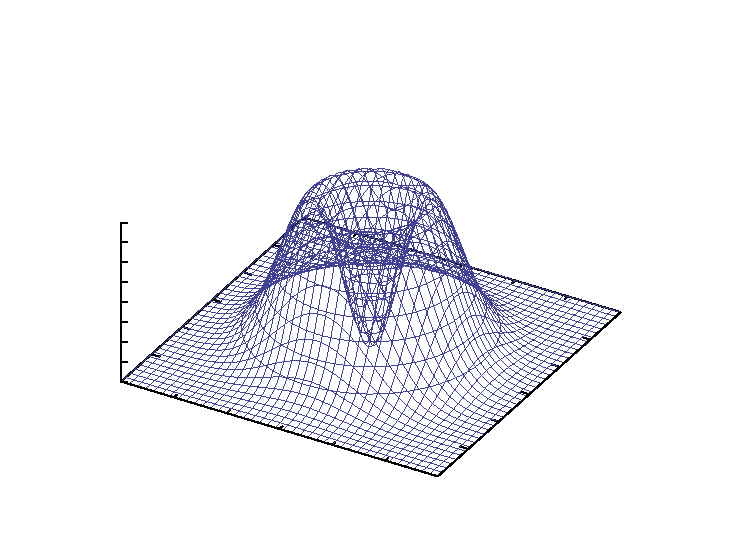
\includegraphics{fig252}}%
    \gplfronttext
  \end{picture}%
\endgroup

 \end{center}
 \caption[]{\quad $f(x,y) = (x^2 + y^2 ) e^{-(x^2 + y^2 )}$.}
 \label{fig:er}
\end{figure}
\end{exmp}
\startexercises\label{sec2dot5}
\probs{A}
\par\noindent For Exercises 1--10, find all local maxima and minima of the function $f(x,y)$.
\begin{enumerate}[\bfseries 1.]
 \begin{multicols}{2}
  \item $f(x,y) = x^3 -3x + y^2$;
  \item $f(x,y) = x^3 -12x+y^2 + 8y$;
 \end{multicols}
 \begin{multicols}{2}
  \item $f(x,y) = x^3 -3x + y^3 -3y$;
  \item $f(x,y) = x^3 + 3x^2 + y^3 -3y^2$;
 \end{multicols}
 \begin{multicols}{2}
  \item $f(x,y) = 2x^3 +6xy + 3y^2$;
  \item $f(x,y) = 2x^3 -6xy + y^2$;
 \end{multicols}
 \begin{multicols}{2}
  \item $f(x,y) = \sqrt{x^2 + y^2}$;
  \item $f(x,y) = x + 2y$;
 \end{multicols}
 \begin{multicols}{2}
  \item $f(x,y) = 4x^2 - 4xy + 2y^2 + 10x - 6y$;
  \item $f(x,y) = -4x^2 + 4xy - 2y^2 + 16x - 12y$.
 \end{multicols}
\suspend{enumerate}
\probs{B}
\resume{enumerate}[{[\bfseries 1.]}]
 \item For a rectangular solid of volume 1000 cubic meters, find the dimensions that will minimize the surface
 area. (\emph{Hint: Use the volume condition to write the surface area as a function of just two variables.})
 \item Prove that if $(x_0,y_0)$ is a local maximum or local minimum point for a smooth function
  $f(x,y)$, then the tangent plane to the surface $z=f(x,y)$ at the point $(x_0,y_0,f(x_0,y_0))$ is parallel to the $xy$-plane.
  (\emph{Hint: Use Theorem \ref{thm:extnec}.})
\suspend{enumerate}
\probs{C}
\resume{enumerate}[{[\bfseries 1.]}]
 \item Find three positive numbers $x$, $y$, $z$ whose sum is 10 such that $x^2 y^2 z$ is a maximum.
\end{enumerate}
\newpage
%Begin Section 2.6
\section{Numerical Methods}
The types of problems that we solved in the previous section were examples of \emph{unconstrained optimization}
problems. That is, we tried to find local (and perhaps even global) maximum and minimum points of real-valued
functions $f(x,y)$, where the points $(x,y)$ could be any points in the domain of $f$. 
The method we used required us to find the critical points of $f$, which meant having to solve the equation
$\nabla f = \textbf{0}$, which in general is a system of two equations in two unknowns ($x$ and $y$). 
While this was relatively simple for the examples we did, in general this will not be the case. 
It might be impossible to solve these equations 
by elementary means.\footnote{This is also a problem
for the equivalent method (the Second Derivative Test) in single-variable calculus, though one that is not usually
emphasized.}

In a situation such as this, the
only choice may be to find a solution using some numerical method which gives a sequence of numbers which
converge to the actual solution. For example, Newton's method for solving equations $f(x) = 0$, which you probably
learned in single-variable calculus. In this section we will describe another method of Newton for
finding critical points of real-valued functions of two variables.

Let $f(x,y)$ be a smooth real-valued function, and define
\begin{displaymath}
 D(x,y) ~=~ \dfrac{\partial^2 f}{\partial x^2}(x,y) \, \dfrac{\partial^2 f}{\partial y^2}(x,y) -
 \biggl( \dfrac{\partial^2 f}{\partial y \, \partial x}(x,y) \biggr)^2 ~.
\end{displaymath}
\textbf{Newton's algorithm}: Pick an initial point $(\ssub{x}{0},\ssub{y}{0})$. For $n = 0, 1, 2, 3, \dots$,
define:
\begin{equation}\label{eqn:newton}
\begin{aligned}
 \ssub{x}{n+1} ~&=~ \ssub{x}{n} -
  \frac{
    \begin{vmatrix}
     \frac{\partial^2 f}{\partial y^2}(\ssub{x}{n},\ssub{y}{n}) &
     \frac{\partial^2 f}{\partial x \, \partial y}(\ssub{x}{n},\ssub{y}{n})\smallskip\\
     \frac{\partial f}{\partial y}(\ssub{x}{n},\ssub{y}{n}) &
     \frac{\partial f}{\partial x}(\ssub{x}{n},\ssub{y}{n})
    \end{vmatrix}}{D(\ssub{x}{n},\ssub{y}{n})} ,
    \\
 \ssub{y}{n+1} ~&=~ \ssub{y}{n} -
  \frac{
    \begin{vmatrix}
     \frac{\partial^2 f}{\partial x^2}(\ssub{x}{n},\ssub{y}{n}) &
     \frac{\partial^2 f}{\partial x \, \partial y}(\ssub{x}{n},\ssub{y}{n})\smallskip\\
     \frac{\partial f}{\partial x}(\ssub{x}{n},\ssub{y}{n}) &
     \frac{\partial f}{\partial y}(\ssub{x}{n},\ssub{y}{n})
    \end{vmatrix}}{D(\ssub{x}{n},\ssub{y}{n})}.
\end{aligned}
\end{equation}
Then the sequence of points $(\ssub{x}{n},\ssub{y}{n})_{n=1}^{\infty}$ typically converges to a critical point. 
If there are several critical points, then you will have to try different initial points to find them.

The choice of the formulas in (\ref{eqn:newton}) is motivated by the following fact, which can be checked by direct calculations.
Assume that the partial derivatives $\tfrac{\partial^2 f}{\partial x^2}(x,y)$, $\tfrac{\partial^2 f}{\partial x\partial y}(x,y)$ and $\tfrac{\partial^2 f}{\partial y^2}(x,y)$ are constants;
in other words, the function $f(x,y)$ can be expressed as a quadratic polynomial in $x$ and $y$, say 
\[f(x,y)=a+bx+cy+lx^2+mxy+ny^2\]
for some constants $a,b,c,l,m,n$.
Then for any choice $(\ssub{x}{0},\ssub{y}{0})$ the formulas (\ref{eqn:newton}) returns a critical point $(\ssub{x}{1},\ssub{y}{1})$, which is unique in this case.

\begin{exmp}
 Find all local maxima and minima of $f(x,y) = x^3 - xy - x + xy^3 - y^4$.\smallskip
 \par\noindent\emph{Solution:} First calculate the necessary partial derivatives:
 \begin{gather*}
  \frac{\partial f}{\partial x} = 3x^2 - y - 1 + y^3 ~, \qquad
  \frac{\partial f}{\partial y} = -x + 3xy^2 - 4y^3\\[6pt]
  \frac{\partial^2 f}{\partial x^2} = 6x ~, \qquad
  \frac{\partial^2 f}{\partial y^2} = 6xy - 12y^2 ~, \qquad
  \frac{\partial^2 f}{\partial y \, \partial x} = -1 + 3y^2
 \end{gather*}
 Notice that solving $\nabla f = \textbf{0}$ would involve solving two third-degree polynomial equations in $x$ and
 $y$, which in this case can not be done easily.
 
 We need to pick an initial point $(\ssub{x}{0},\ssub{y}{0})$ for our algorithm. Looking at the graph of
 $z = f(x,y)$ over a large region may help (see Figure \ref{fig:newtonbig} below), though it may be hard to tell
 where the critical points are.
\begin{figure}[h]
 \begin{center}
  % GNUPLOT: LaTeX picture with Postscript
\begingroup
\footnotesize
  \makeatletter
  \providecommand\color[2][]{%
    \GenericError{(gnuplot) \space\space\space\@spaces}{%
      Package color not loaded in conjunction with
      terminal option `colourtext'%
    }{See the gnuplot documentation for explanation.%
    }{Either use 'blacktext' in gnuplot or load the package
      color.sty in LaTeX.}%
    \renewcommand\color[2][]{}%
  }%
  \providecommand\includegraphics[2][]{%
    \GenericError{(gnuplot) \space\space\space\@spaces}{%
      Package graphicx or graphics not loaded%
    }{See the gnuplot documentation for explanation.%
    }{The gnuplot epslatex terminal needs graphicx.sty or graphics.sty.}%
    \renewcommand\includegraphics[2][]{}%
  }%
  \providecommand\rotatebox[2]{#2}%
  \@ifundefined{ifGPcolor}{%
    \newif\ifGPcolor
    \GPcolortrue
  }{}%
  \@ifundefined{ifGPblacktext}{%
    \newif\ifGPblacktext
    \GPblacktexttrue
  }{}%
  % define a \g@addto@macro without @ in the name:
  \let\gplgaddtomacro\g@addto@macro
  % define empty templates for all commands taking text:
  \gdef\gplbacktext{}%
  \gdef\gplfronttext{}%
  \makeatother
  \ifGPblacktext
    % no textcolor at all
    \def\colorrgb#1{}%
    \def\colorgray#1{}%
  \else
    % gray or color?
    \ifGPcolor
      \def\colorrgb#1{\color[rgb]{#1}}%
      \def\colorgray#1{\color[gray]{#1}}%
      \expandafter\def\csname LTw\endcsname{\color{white}}%
      \expandafter\def\csname LTb\endcsname{\color{black}}%
      \expandafter\def\csname LTa\endcsname{\color{black}}%
      \expandafter\def\csname LT0\endcsname{\color[rgb]{1,0,0}}%
      \expandafter\def\csname LT1\endcsname{\color[rgb]{0,1,0}}%
      \expandafter\def\csname LT2\endcsname{\color[rgb]{0,0,1}}%
      \expandafter\def\csname LT3\endcsname{\color[rgb]{1,0,1}}%
      \expandafter\def\csname LT4\endcsname{\color[rgb]{0,1,1}}%
      \expandafter\def\csname LT5\endcsname{\color[rgb]{1,1,0}}%
      \expandafter\def\csname LT6\endcsname{\color[rgb]{0,0,0}}%
      \expandafter\def\csname LT7\endcsname{\color[rgb]{1,0.3,0}}%
      \expandafter\def\csname LT8\endcsname{\color[rgb]{0.5,0.5,0.5}}%
    \else
      % gray
      \def\colorrgb#1{\color{black}}%
      \def\colorgray#1{\color[gray]{#1}}%
      \expandafter\def\csname LTw\endcsname{\color{white}}%
      \expandafter\def\csname LTb\endcsname{\color{black}}%
      \expandafter\def\csname LTa\endcsname{\color{black}}%
      \expandafter\def\csname LT0\endcsname{\color{black}}%
      \expandafter\def\csname LT1\endcsname{\color{black}}%
      \expandafter\def\csname LT2\endcsname{\color{black}}%
      \expandafter\def\csname LT3\endcsname{\color{black}}%
      \expandafter\def\csname LT4\endcsname{\color{black}}%
      \expandafter\def\csname LT5\endcsname{\color{black}}%
      \expandafter\def\csname LT6\endcsname{\color{black}}%
      \expandafter\def\csname LT7\endcsname{\color{black}}%
      \expandafter\def\csname LT8\endcsname{\color{black}}%
    \fi
  \fi
  \setlength{\unitlength}{0.0500bp}%
  \begin{picture}(6802.00,5040.00)%
    \gplgaddtomacro\gplbacktext{%
      \csname LTb\endcsname%
      \put(5969,2116){\makebox(0,0)[l]{\strut{}-20}}%
      \put(5749,1919){\makebox(0,0)[l]{\strut{}-15}}%
      \put(5530,1722){\makebox(0,0)[l]{\strut{}-10}}%
      \put(5310,1525){\makebox(0,0)[l]{\strut{}-5}}%
      \put(5091,1328){\makebox(0,0)[l]{\strut{} 0}}%
      \put(4871,1131){\makebox(0,0)[l]{\strut{} 5}}%
      \put(4652,934){\makebox(0,0)[l]{\strut{} 10}}%
      \put(4432,736){\makebox(0,0)[l]{\strut{} 15}}%
      \put(4212,539){\makebox(0,0)[l]{\strut{} 20}}%
      \put(936,1435){\makebox(0,0){\strut{}-20}}%
      \put(1316,1321){\makebox(0,0){\strut{}-15}}%
      \put(1697,1208){\makebox(0,0){\strut{}-10}}%
      \put(2077,1094){\makebox(0,0){\strut{}-5}}%
      \put(2457,980){\makebox(0,0){\strut{} 0}}%
      \put(2838,866){\makebox(0,0){\strut{} 5}}%
      \put(3218,753){\makebox(0,0){\strut{} 10}}%
      \put(3597,639){\makebox(0,0){\strut{} 15}}%
      \put(3977,525){\makebox(0,0){\strut{} 20}}%
      \put(876,1534){\makebox(0,0)[r]{\strut{}-350000}}%
      \put(876,1725){\makebox(0,0)[r]{\strut{}-300000}}%
      \put(876,1916){\makebox(0,0)[r]{\strut{}-250000}}%
      \put(876,2106){\makebox(0,0)[r]{\strut{}-200000}}%
      \put(876,2297){\makebox(0,0)[r]{\strut{}-150000}}%
      \put(876,2488){\makebox(0,0)[r]{\strut{}-100000}}%
      \put(876,2678){\makebox(0,0)[r]{\strut{}-50000}}%
      \put(876,2869){\makebox(0,0)[r]{\strut{} 0}}%
      \put(876,3060){\makebox(0,0)[r]{\strut{} 50000}}%
      \put(959,3443){\makebox(0,0){\strut{}$z$}}%
    }%
    \gplgaddtomacro\gplfronttext{%
      \csname LTb\endcsname%
      \put(5682,1184){\makebox(0,0){\strut{}$x$}}%
      \put(2084,685){\makebox(0,0){\strut{}$y$}}%
      \put(959,3443){\makebox(0,0){\strut{}$z$}}%
    }%
    \gplbacktext
    \put(0,0){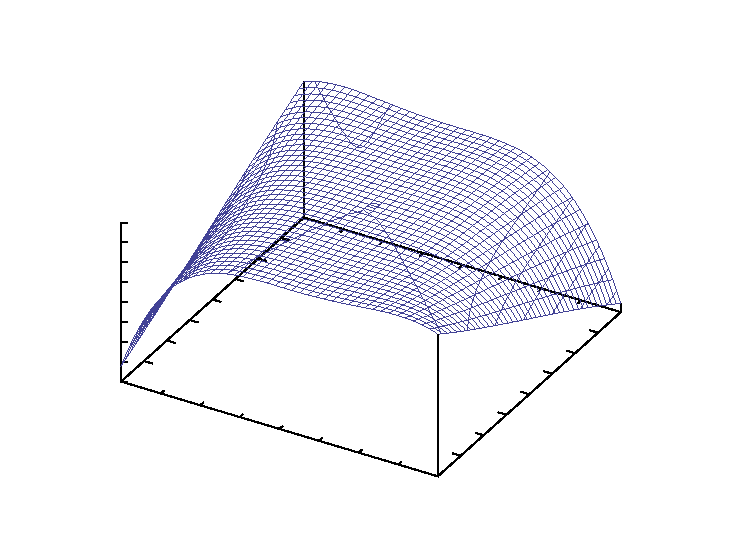
\includegraphics{fig261}}%
    \gplfronttext
  \end{picture}%
\endgroup

 \end{center}
 \caption[]{\quad $f(x,y) = x^3 - xy - x + xy^3 - y^4$ for $-20 \le x \le 20$ and $-20 \le y \le 20$.}
 \label{fig:newtonbig}
\end{figure}

Notice in the formulas (\ref{eqn:newton}) that we divide by $D$, so we should pick an initial point where $D$ is not
zero. And we can see that $D(0,0) = (0)(0) - (-1)^2 = -1 \ne 0$, so take $(0,0)$ as our initial point. Since it may
take a large number of iterations of Newton's algorithm to be sure that we are close enough to the actual critical
point, and since the computations are quite tedious, we will let a computer do the computing. For this, we will
write a simple program, using the Java programming language, which will take a given initial point as a parameter
and then perform 100 iterations of Newton's algorithm. In each iteration the new point will be printed, so that we
can see if there is convergence. The full code is shown in Listing \ref{java}.

\definecolor{codecolor}{HTML}{FFF7E0}
\lstset{language=Java,showstringspaces=false,
basicstyle={\small\fontfamily{fvm}\fontseries{m}\selectfont},
columns=fullflexible,backgroundcolor=\color{codecolor},
commentstyle={\color{blue}\small\fontfamily{fvm}\itshape\selectfont},
keywordstyle={\small\fontfamily{fvm}\fontseries{b}\selectfont},keepspaces=true,
float=h,caption={\hspace{1em}Program listing for newton.java},label=java,stringstyle=\color{red},
frame=single,aboveskip=\medskipamount,belowskip=\medskipamount,captionpos=b}
\begin{lstlisting}
//Program to find the critical points of f(x,y)=x^3-xy-x+xy^3-y^4
public class newton {
 public static void main(String[] args) {
   //Get the initial point (x,y) as command-line parameters
   double x = Double.parseDouble(args[0]); //Initial x value
   double y = Double.parseDouble(args[1]); //Initial y value
   System.out.println("Initial point: (" + x + "," + y + ")");
   //Go through 100 iterations of Newton's algorithm
   for (int n=1; n<=100; n++) {
      double D = fxx(x,y)*fyy(x,y) - Math.pow(fxy(x,y),2);
      double xn = x; double yn = y; //The current x and y values
      if (D == 0) { //We can not divide by 0
         System.out.println("Error: D = 0 at iteration n = " + n);
         System.exit(0); //End the program
      } else { //Calculate the new values for x and y
         x = xn - (fyy(xn,yn)*fx(xn,yn) - fxy(xn,yn)*fy(xn,yn))/D;
         y = yn - (fxx(xn,yn)*fy(xn,yn) - fxy(xn,yn)*fx(xn,yn))/D;
         System.out.println("n = " + n + ": (" + x + "," + y + ")");
      }
   }
 }
 //Below are the parts specific to the function f
 //The first partial derivative of f wrt x: 3x^2-y-1+y^3
 public static double fx(double x, double y) {
   return 3*Math.pow(x,2) - y - 1 + Math.pow(y,3);
 }
 //The first partial derivative of f wrt y: -x+3xy^2-4y^3
 public static double fy(double x, double y) {
   return -x + 3*x*Math.pow(y,2) - 4*Math.pow(y,3);
 }
 //The second partial derivative of f wrt x: 6x
 public static double fxx(double x, double y) {
   return 6*x;
 }
 //The second partial derivative of f wrt y: 6xy-12y^2
 public static double fyy(double x, double y) {
   return 6*x*y - 12*Math.pow(y,2);
 }
 //The mixed second partial derivative of f wrt x and y: -1+3y^2
 public static double fxy(double x, double y) {
   return -1 + 3*Math.pow(y,2);
 }
}
\end{lstlisting}

To use this program, you should first save the code in Listing \ref{java} in a plain text file called
\texttt{newton.java}. You will need the Java Development Kit\footnote{Available for free at
\texttt{http://www.oracle.com/technetwork/java/javase/downloads/}} to compile the code. In the directory where \texttt{newton.java} is
saved, run this command at a command prompt to compile the code: \texttt{javac newton.java}\\
Then run the program with the initial point $(0,0)$ with this command:\\\texttt{java newton 0 0}

Below is the output of the program using $(0,0)$ as the initial point, truncated to show the first 10 lines and
the last 5 lines:

\begin{verbatim}
java newton 0 0
Initial point: (0.0,0.0)
n = 1: (0.0,-1.0)
n = 2: (1.0,-0.5)
n = 3: (0.6065857885615251,-0.44194107452339687)
n = 4: (0.484506572966545,-0.405341511995805)
n = 5: (0.47123972682634485,-0.3966334583092305)
n = 6: (0.47113558510349535,-0.39636450001936047)
n = 7: (0.4711356343449705,-0.3963643379632247)
n = 8: (0.4711356343449874,-0.39636433796318005)
n = 9: (0.4711356343449874,-0.39636433796318005)
n = 10: (0.4711356343449874,-0.39636433796318005)
...
n = 96: (0.4711356343449874,-0.39636433796318005)
n = 97: (0.4711356343449874,-0.39636433796318005)
n = 98: (0.4711356343449874,-0.39636433796318005)
n = 99: (0.4711356343449874,-0.39636433796318005)
n = 100: (0.4711356343449874,-0.39636433796318005)
\end{verbatim}

As you can see, we appear to have converged fairly quickly (after only 8 iterations) to what appears to be an actual
critical point (up to Java's level of precision), namely the point
$(0.4711356343449874,-0.39636433796318005)$. It is easy to confirm that $\nabla f = \textbf{0}$ at this point,
either by evaluating $\frac{\partial f}{\partial x}$ and $\frac{\partial f}{\partial y}$ at the point ourselves or by
modifying our program to also print the values of the partial derivatives at the point. It turns out that
both partial derivatives are indeed close enough to zero to be considered zero:
\begin{gather*}
 \frac{\partial f}{\partial x}(0.4711356343449874,-0.39636433796318005) = 4.85722573273506 \times 10^{-17}\smallskip\\
 \frac{\partial f}{\partial y}(0.4711356343449874,-0.39636433796318005) = -8.326672684688674 \times 10^{-17}
\end{gather*}
We also have $D(0.4711356343449874,-0.39636433796318005) = -8.776075636032301 < 0$, so by
Theorem \ref{thm:extsuff} we know that $(0.4711356343449874,-0.39636433796318005)$ is a saddle point.

Since $\nabla f$ consists of cubic polynomials, it seems likely that there may be three critical points.
The computer program makes experimenting with other initial points easy, and trying different values does indeed lead
to different sequences which converge:

\begin{verbatim}
java newton -1 -1
Initial point: (-1.0,-1.0)
n = 1: (-0.5,-0.5)
n = 2: (-0.49295774647887325,-0.08450704225352113)
n = 3: (-0.1855674752461383,-1.2047647348546167)
n = 4: (-0.4540060574531383,-0.8643989895639324)
n = 5: (-0.3672160534444,-0.5426077421319053)
n = 6: (-0.4794622222856417,-0.24529117721011612)
n = 7: (0.11570743992954591,-2.4319791238981274)
n = 8: (-0.05837851765533317,-1.6536079835854451)
n = 9: (-0.129841298650007,-1.121516233310142)
n = 10: (-1.004453014967208,-0.9206128022529645)
n = 11: (-0.5161209914612475,-0.4176293491131443)
n = 12: (-0.5788664043863884,0.2918236503332734)
n = 13: (-0.6985177124230715,0.49848120123515316)
n = 14: (-0.6733618916578702,0.4345777963475479)
n = 15: (-0.6704392913413444,0.4252025996474051)
n = 16: (-0.6703832679150286,0.4250147307973365)
n = 17: (-0.6703832459238701,0.42501465652421205)
n = 18: (-0.6703832459238667,0.4250146565242004)
n = 19: (-0.6703832459238667,0.42501465652420045)
n = 20: (-0.6703832459238667,0.42501465652420045)
...
n = 98: (-0.6703832459238667,0.42501465652420045)
n = 99: (-0.6703832459238667,0.42501465652420045)
n = 100: (-0.6703832459238667,0.42501465652420045)
\end{verbatim}

Again, it is easy to confirm that both $\frac{\partial f}{\partial x}$ and $\frac{\partial f}{\partial y}$ vanish
at the point\\$(-0.6703832459238667,0.42501465652420045)$, which means it is a critical point. 
And
\begin{gather*}
 D(-0.6703832459238667,0.42501465652420045) = 15.3853578526055 > 0\\
 \frac{\partial^2 f}{\partial x^2}(-0.6703832459238667,0.42501465652420045) = -4.0222994755432 < 0
\end{gather*}
so we know that $(-0.6703832459238667,0.42501465652420045)$ is a local maximum. An idea of what the graph of $f$ looks
like near that point is shown in Figure \ref{fig:newtonmax}, which does suggest a local maximum around that point.

\begin{figure}[h]
 \begin{center}
  % GNUPLOT: LaTeX picture with Postscript
\begingroup
\footnotesize
  \makeatletter
  \providecommand\color[2][]{%
    \GenericError{(gnuplot) \space\space\space\@spaces}{%
      Package color not loaded in conjunction with
      terminal option `colourtext'%
    }{See the gnuplot documentation for explanation.%
    }{Either use 'blacktext' in gnuplot or load the package
      color.sty in LaTeX.}%
    \renewcommand\color[2][]{}%
  }%
  \providecommand\includegraphics[2][]{%
    \GenericError{(gnuplot) \space\space\space\@spaces}{%
      Package graphicx or graphics not loaded%
    }{See the gnuplot documentation for explanation.%
    }{The gnuplot epslatex terminal needs graphicx.sty or graphics.sty.}%
    \renewcommand\includegraphics[2][]{}%
  }%
  \providecommand\rotatebox[2]{#2}%
  \@ifundefined{ifGPcolor}{%
    \newif\ifGPcolor
    \GPcolortrue
  }{}%
  \@ifundefined{ifGPblacktext}{%
    \newif\ifGPblacktext
    \GPblacktexttrue
  }{}%
  % define a \g@addto@macro without @ in the name:
  \let\gplgaddtomacro\g@addto@macro
  % define empty templates for all commands taking text:
  \gdef\gplbacktext{}%
  \gdef\gplfronttext{}%
  \makeatother
  \ifGPblacktext
    % no textcolor at all
    \def\colorrgb#1{}%
    \def\colorgray#1{}%
  \else
    % gray or color?
    \ifGPcolor
      \def\colorrgb#1{\color[rgb]{#1}}%
      \def\colorgray#1{\color[gray]{#1}}%
      \expandafter\def\csname LTw\endcsname{\color{white}}%
      \expandafter\def\csname LTb\endcsname{\color{black}}%
      \expandafter\def\csname LTa\endcsname{\color{black}}%
      \expandafter\def\csname LT0\endcsname{\color[rgb]{1,0,0}}%
      \expandafter\def\csname LT1\endcsname{\color[rgb]{0,1,0}}%
      \expandafter\def\csname LT2\endcsname{\color[rgb]{0,0,1}}%
      \expandafter\def\csname LT3\endcsname{\color[rgb]{1,0,1}}%
      \expandafter\def\csname LT4\endcsname{\color[rgb]{0,1,1}}%
      \expandafter\def\csname LT5\endcsname{\color[rgb]{1,1,0}}%
      \expandafter\def\csname LT6\endcsname{\color[rgb]{0,0,0}}%
      \expandafter\def\csname LT7\endcsname{\color[rgb]{1,0.3,0}}%
      \expandafter\def\csname LT8\endcsname{\color[rgb]{0.5,0.5,0.5}}%
    \else
      % gray
      \def\colorrgb#1{\color{black}}%
      \def\colorgray#1{\color[gray]{#1}}%
      \expandafter\def\csname LTw\endcsname{\color{white}}%
      \expandafter\def\csname LTb\endcsname{\color{black}}%
      \expandafter\def\csname LTa\endcsname{\color{black}}%
      \expandafter\def\csname LT0\endcsname{\color{black}}%
      \expandafter\def\csname LT1\endcsname{\color{black}}%
      \expandafter\def\csname LT2\endcsname{\color{black}}%
      \expandafter\def\csname LT3\endcsname{\color{black}}%
      \expandafter\def\csname LT4\endcsname{\color{black}}%
      \expandafter\def\csname LT5\endcsname{\color{black}}%
      \expandafter\def\csname LT6\endcsname{\color{black}}%
      \expandafter\def\csname LT7\endcsname{\color{black}}%
      \expandafter\def\csname LT8\endcsname{\color{black}}%
    \fi
  \fi
  \setlength{\unitlength}{0.0500bp}%
  \begin{picture}(6802.00,5040.00)%
    \gplgaddtomacro\gplbacktext{%
      \csname LTb\endcsname%
      \put(5969,2116){\makebox(0,0)[l]{\strut{}-1}}%
      \put(5618,1800){\makebox(0,0)[l]{\strut{}-0.8}}%
      \put(5266,1485){\makebox(0,0)[l]{\strut{}-0.6}}%
      \put(4915,1170){\makebox(0,0)[l]{\strut{}-0.4}}%
      \put(4564,855){\makebox(0,0)[l]{\strut{}-0.2}}%
      \put(4212,539){\makebox(0,0)[l]{\strut{} 0}}%
      \put(936,1435){\makebox(0,0){\strut{} 0}}%
      \put(1545,1253){\makebox(0,0){\strut{} 0.2}}%
      \put(2153,1071){\makebox(0,0){\strut{} 0.4}}%
      \put(2761,889){\makebox(0,0){\strut{} 0.6}}%
      \put(3370,707){\makebox(0,0){\strut{} 0.8}}%
      \put(3977,525){\makebox(0,0){\strut{} 1}}%
      \put(876,1534){\makebox(0,0)[r]{\strut{}-1}}%
      \put(876,1725){\makebox(0,0)[r]{\strut{}-0.8}}%
      \put(876,1916){\makebox(0,0)[r]{\strut{}-0.6}}%
      \put(876,2106){\makebox(0,0)[r]{\strut{}-0.4}}%
      \put(876,2297){\makebox(0,0)[r]{\strut{}-0.2}}%
      \put(876,2488){\makebox(0,0)[r]{\strut{} 0}}%
      \put(876,2678){\makebox(0,0)[r]{\strut{} 0.2}}%
      \put(876,2869){\makebox(0,0)[r]{\strut{} 0.4}}%
      \put(876,3060){\makebox(0,0)[r]{\strut{} 0.6}}%
      \put(300,2343){\makebox(0,0){\strut{}$z$}}%
    }%
    \gplgaddtomacro\gplfronttext{%
      \csname LTb\endcsname%
      \put(5682,1184){\makebox(0,0){\strut{}$x$}}%
      \put(2084,685){\makebox(0,0){\strut{}$y$}}%
      \put(300,2343){\makebox(0,0){\strut{}$z$}}%
      \put(3487,3846){\makebox(0,0)[l]{\strut{}$(-0.67,0.42,0.57)$}}%
    }%
    \gplbacktext
    \put(0,0){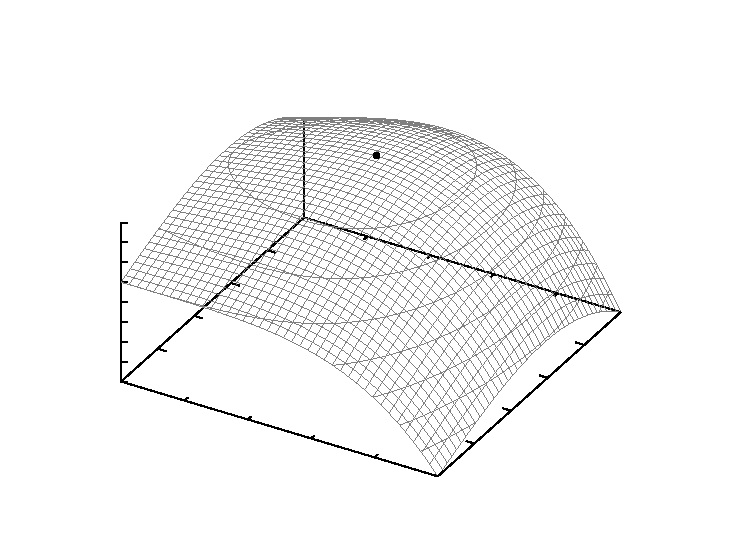
\includegraphics{fig262}}%
    \gplfronttext
  \end{picture}%
\endgroup

 \end{center}
 \caption[]{\quad $f(x,y) = x^3 - xy - x + xy^3 - y^4$ for $-1 \le x \le 0$ and $0 \le y \le 1$.}
 \label{fig:newtonmax}
\end{figure}

Finally, running the computer program with the initial point $(-5,-5)$ yields the critical point
$(-7.540962756992551,-5.595509445899435)$, with $D < 0$ at that point, which makes it a saddle point.

We can summarize our findings for the function $f(x,y) = x^3 - xy - x + xy^3 - y^4$:
\begin{align*}
 (0.4711356343449874,-0.39636433796318005)&:~ \text{saddle point}\\
 (-0.6703832459238667,0.42501465652420045)&:~ \text{local maximum}\\
 (-7.540962756992551,-5.595509445899435)&:~ \text{saddle point}
\end{align*}
\end{exmp}
\hrule width \textwidth height 0.5pt
\medskip

The derivation of Newton's algorithm, and the proof that it converges (given a ``reasonable'' choice for the
initial point) requires techniques beyond the scope of this text. See \cite{rr} for more
detail and for discussion of other numerical methods. Our description of Newton's algorithm is the special
two-variable case of a more general algorithm that can be applied to functions of $n \ge 2$ variables.

In the case of functions which have a global maximum or minimum, 
Newton's algorithm can be used to find those points. 
In general, global maxima and minima tend to be more interesting than local versions, at least in practical applications. 
A maximization problem can always be turned into a minimization problem (why?), so a large number of methods have been developed to find the global minimum of functions of any number of variables. 
This field of study is called \emph{nonlinear programming}. 

Many of these methods are based on the \emph{steepest
descent} technique, which is based on an idea that we discussed in Section 2.4. Recall that the negative gradient
$-\nabla f$ gives the direction of the fastest rate of decrease of a function $f$. 
The crux of the steepest descent idea, then, is that starting from some initial point, you move a certain amount in the direction of $-\nabla f$ at that point. 
Wherever that takes you becomes your new point, and you then just keep repeating that procedure until
eventually (hopefully) you reach the point where $f$ has its smallest value. There is a ``pure'' steepest descent
method, and a multitude of variations on it that improve the rate of convergence, ease of calculation, etc. 
For more discussion of this, and of nonlinear programming in general, see \cite{bss}.\index{steepest descent}
\startexercises\label{sec2dot6}
\probs{C}\smallskip
\begin{enumerate}[\bfseries 1.]
 \item Recall Example \ref{exmp:globalmin} from the previous section, where we showed that the point $(2,1)$ was a global minimum for the function $f(x,y) = (x-2)^4 + (x-2y)^2$. 
 Notice that our computer program can be modified fairly easily to use this function (just change the return values in the fx, fy, fxx, fyy and fxy
  function definitions to use the appropriate
  partial derivative). Either modify that program or write one of your own in a programming language of your
  choice to show that Newton's algorithm does lead to the point $(2,1)$. First use the initial point $(0,3)$, then use
  the initial point $(3,2)$, and compare the results. Make sure that your program attempts to do 100 iterations of the
  algorithm. Did anything strange happen when your program ran? If so, how do you explain it? (\emph{Hint: Something
  strange should happen.})
 \item There is a version of Newton's algorithm for solving a system of two equations
  \begin{displaymath}
   \ssub{f}{1}(x,y) = 0 \qquad\text{and}\qquad \ssub{f}{2}(x,y) = 0 ~,
  \end{displaymath}
  where $\ssub{f}{1}(x,y)$ and $\ssub{f}{2}(x,y)$ are smooth real-valued functions:\\
  Pick an initial point $(\ssub{x}{0},\ssub{y}{0})$. For $n = 0, 1, 2, 3, \dots$, define:
  \begin{gather*}
   \ssub{x}{n+1} ~=~ \ssub{x}{n} -
   \frac{
    \begin{vmatrix}
     \ssub{f}{1}(\ssub{x}{n},\ssub{y}{n}) &
     \ssub{f}{2}(\ssub{x}{n},\ssub{y}{n})\smallskip\\
     \frac{\partial \ssub{f}{1}}{\partial y}(\ssub{x}{n},\ssub{y}{n}) &
     \frac{\partial \ssub{f}{2}}{\partial y}(\ssub{x}{n},\ssub{y}{n})
    \end{vmatrix}}{D(\ssub{x}{n},\ssub{y}{n})} ~,\quad
   \ssub{y}{n+1} ~=~ \ssub{y}{n} +
   \frac{
    \begin{vmatrix}
     \ssub{f}{1}(\ssub{x}{n},\ssub{y}{n}) &
     \ssub{f}{2}(\ssub{x}{n},\ssub{y}{n})\smallskip\\
     \frac{\partial \ssub{f}{1}}{\partial x}(\ssub{x}{n},\ssub{y}{n}) &
     \frac{\partial \ssub{f}{2}}{\partial x}(\ssub{x}{n},\ssub{y}{n})
    \end{vmatrix}}{D(\ssub{x}{n},\ssub{y}{n})} ~~,~\text{where}\\[6pt]
    D(\ssub{x}{n},\ssub{y}{n}) ~=~ \frac{\partial \ssub{f}{1}}{\partial x}(\ssub{x}{n},\ssub{y}{n})\,
    \frac{\partial \ssub{f}{2}}{\partial y}(\ssub{x}{n},\ssub{y}{n}) -
    \frac{\partial \ssub{f}{1}}{\partial y}(\ssub{x}{n},\ssub{y}{n})\,
    \frac{\partial \ssub{f}{2}}{\partial x}(\ssub{x}{n},\ssub{y}{n}) ~.
  \end{gather*}
  Then the sequence of points $(\ssub{x}{n},\ssub{y}{n})_{n=1}^{\infty}$ converges to a solution. Write a computer
  program that uses this algorithm to find approximate solutions to the system of equations
  \begin{displaymath}
   \ssub{f}{1}(x,y) = \sin(xy)-x-y=0 \qquad\text{and}\qquad \ssub{f}{2}(x,y) = e^{2x}-2x+3y=0 ~.
  \end{displaymath}
  Show that you get two different solutions when using $(0,0)$ and $(1,1)$ for the initial point
  $(\ssub{x}{0},\ssub{y}{0})$.
\end{enumerate}
\newpage
%Begin Section 2.7
\section{Lagrange Multipliers}
In Sections 2.5 and 2.6 we were concerned with finding maxima and minima of functions without any constraints on
the variables (other than being in the domain of the function). What would we do if there were constraints on the
variables? The following example illustrates a simple case of this type of problem.\index{Lagrange multiplier}

\medskip
\hrule width \textwidth height 0.5pt
\begin{exmp}\label{exmp:consimple}
 For a rectangle whose perimeter is $20$ m, find the dimensions that will maximize the area.\smallskip
 \par\noindent \emph{Solution:} The area $A$ of a rectangle with width $x$ and height $y$ is $A = xy$. The perimeter $P$
 of the rectangle is then given by the formula $P = 2x + 2y$. Since we are given that the perimeter $P = 20$, this
 problem can be stated as:
 \begin{align*}
  \text{Maximize}&: ~ f(x,y) = xy\\
  \text{given}&: ~ 2x + 2y = 20
 \end{align*}
 The reader is probably familiar with a simple method, using single-variable calculus, for solving this problem. Since
 we must have $2x+2y=20$, then we can solve for, say, $y$ in terms of $x$ using that equation. This gives $y = 10 - x$,
 which we then substitute into $f$ to get $f(x,y) = xy = x(10-x) = 10x - x^2$. 
 This is now a function of $x$ alone, so
 we now just have to maximize the function $f(x) = 10x - x^2$ on the interval $\lbrack 0, 10 \rbrack$. Since
 $f\,'(x) = 10-2x = 0 \Rightarrow x =5$ and $f\,''(5) = -2 < 0$, then the Second Derivative Test tells us that $x=5$ is
 a local maximum for $f$, and hence $x=5$ must be the global maximum on the interval $\lbrack 0, 10 \rbrack$ (since
 $f = 0$ at the endpoints of the interval). 
 So since $y=10-x =5$, then the maximum area occurs for a rectangle whose
 width and height both are $5$ m.
\end{exmp}
\hrule width \textwidth height 0.5pt
\medskip

Notice in the above example that the ease of the solution depended on being able to solve for one variable in terms of the other in the equation $2x+2y=20$. 
But what if that were not possible (which is often the case)?
In this section we will use a general method, called the
\emph{Lagrange multiplier method}\footnote{Named after the French mathematician Joseph Louis Lagrange (1736--1813).}, for
solving \emph{constrained optimization} problems:
\begin{align*}
 \text{Maximize (or minimize)}&: ~ f(x,y) ~~\text{(or $f(x,y,z)$)}\\
 \text{given}&: ~ g(x,y) = c ~~\text{(or $g(x,y,z) = c$) for some constant $c$}
\end{align*}
The equation $g(x,y) = c$ is called the \emph{constraint equation}, and we say that $x$ and $y$ are \emph{constrained}
by $g(x,y) = c$. Points $(x,y)$ which are maxima or minima of $f(x,y)$ with the condition that they satisfy
the constraint equation $g(x,y)=c$ are called \emph{constrained maximum} or \emph{constrained minimum} points,
respectively. Similar definitions hold for functions of three variables.\index{constrained critical point}

The Lagrange multiplier method for solving such problems can now be stated:

\statethm{thm:lagrange}{
 {Let $f(x,y)$ and $g(x,y)$ be smooth functions, and suppose that $c$ is a scalar constant such
 that $\nabla g(x,y) \ne \textbf{0}$ for all $(x,y)$ that satisfy the equation $g(x,y) = c$. Then to solve the
 constrained optimization problem
 \begin{align*}
  \text{Maximize (or minimize)}&: ~ f(x,y)\\
  \text{given}&: ~ g(x,y) = c ~,
 \end{align*}
 find the points $(x,y)$ that solve the equation $\nabla f(x,y) = \lambda \nabla g(x,y)$ for some constant
 $\lambda$ (the number $\lambda$ is called the \emph{Lagrange multiplier}). If there is a constrained maximum or
 minimum, then it must be such a point.}
}

A rigorous proof of the above theorem requires use of the Implicit Function Theorem, which is beyond the scope of this
text.\footnote{See \cite[\S\,6.8]{tm} for more detail.} Note that the theorem only gives a \emph{necessary} condition
for a point to be a constrained maximum or minimum. Whether a point $(x,y)$ that satisfies
$\nabla f(x,y) = \lambda \nabla g(x,y)$ for some $\lambda$ actually \emph{is} a constrained maximum or minimum can
\emph{sometimes} be determined by the nature of the problem itself. For instance, in Example \ref{exmp:consimple} it was
clear that there had to be a global maximum.

So how can you tell when a point that satisfies the condition in Theorem \ref{thm:lagrange} really is a
constrained maximum or minimum? The answer is that it depends on the constraint function $g(x,y)$, together with any
implicit constraints. 
It can be shown\footnote{Again, see \cite{tm}.} that if the constraint equation $g(x,y)=c$  as above describes a \emph{bounded} set $B$ in $\Real{2}$, then the constrained maximum or minimum of
$f(x,y)$ will occur at a point $(x,y)$ satisfying $\nabla f(x,y) = \lambda \nabla g(x,y)$.

Even if the set described by equaiton $g(x,y)=c$ is not bounded, 
the problem might contain some ``hidden constraints'' so that the minimum (or maximu) should be taken on a bounded  set.

Say in the Example \ref{exmp:consimple} the constraint equation $2x+2y=20$ describes a line in $\Real{2}$, which by itself is
not bounded.
However, there are ``hidden'' constraints, due to the nature of the problem, namely $0\le x,y \le 10$,
which cause that line to be restricted to a \emph{line segment} in $\Real{2}$, which \emph{is} bounded;
the the endpoints of that line
segment form the ``boundary''.

In a general case of that type the maximum or minimum of
$f(x,y)$ will occur either at a point $(x,y)$ satisfying $\nabla f(x,y) = \lambda \nabla g(x,y)$  or at a ``boundary''
point of the set described by the hidden constraints.

\medskip
\hrule width \textwidth height 0.5pt
\begin{exmp}\label{exmp:rectlm}
 For a rectangle whose perimeter is $20$ m, use the Lagrange multiplier method to find the dimensions that will
 maximize the area.\smallskip
 \par\noindent \emph{Solution:} As we saw in Example \ref{exmp:consimple}, with $x$ and $y$ representing the width and
  height, respectively, of the rectangle, this problem can be stated as:
 \begin{align*}
  \text{Maximize}&: ~ f(x,y) = xy\\
  \text{given}&: ~ g(x,y) = 2x + 2y = 20
 \end{align*}
 Then solving the equation $\nabla f(x,y) = \lambda \nabla g(x,y)$ for some $\lambda$ means solving the equations
 \[\dfrac{\partial f}{\partial x} = \lambda \dfrac{\partial g}{\partial x}
  \quad
\text{and}
\quad
 \dfrac{\partial f}{\partial y} = \lambda \dfrac{\partial g}{\partial y},\] namely:
 \begin{align*}
  y ~&=~ 2\lambda ~,\\
  x ~&=~ 2\lambda
 \end{align*}
 The general idea is to solve for $\lambda$ in both equations, then set those expressions equal (since they both equal
 $\lambda$) to solve for $x$ and $y$. Doing this we get
 \begin{displaymath}
  \frac{y}{2} ~=~ \lambda ~=~ \frac{x}{2} \quad \Rightarrow \quad x = y ~,
 \end{displaymath}
 so now substitute either of the expressions for $x$ or $y$ into the constraint equation to solve for $x$ and $y$:
 \begin{displaymath}
  20 ~=~ g(x,y) ~=~ 2x + 2y ~= ~2x + 2x ~=~ 4x \quad \Rightarrow \quad x = 5 \quad \Rightarrow \quad y = 5
 \end{displaymath}
 There must be a maximum area, since the minimum area is $0$ and $f(5,5) = 25 > 0$, so the point $(5,5)$ that we found
 (called a \emph{constrained critical point}) must be the constrained maximum.\\
 $\therefore ~$ 
 The maximum area occurs for a rectangle whose width and height both are $5$ m.
\end{exmp}
\hrule width \textwidth height 0.5pt
\begin{exmp}
 Find the points on the circle $x^2 + y^2 = 80$ which are closest to and farthest from the point $(1,2)$.\smallskip
 \par\noindent \emph{Solution:} The distance $d$ from any point $(x,y)$ to the point $(1,2)$ is
 \begin{displaymath}
  d = \sqrt{(x-1)^2 + (y-2)^2} ~,
 \end{displaymath}
 and minimizing the distance is equivalent to minimizing the square of the distance. Thus the problem can be stated as:
 \begin{align*}
  \text{Maximize (and minimize)}&: ~ f(x,y) = (x-1)^2 + (y-2)^2\\
  \text{given}&: ~ g(x,y) = x^2 + y^2 = 80
 \end{align*}
 Solving $\nabla f(x,y) = \lambda \nabla g(x,y)$ means solving the following equations:
 \begin{align*}
  2(x-1) ~&=~ 2\lambda x ~,\\
  2(y-2) ~&=~ 2\lambda y
 \end{align*}
 Note that $x \ne 0$ since otherwise we would get $-2=0$ in the first equation. Similarly, $y \ne 0$.
 So we can solve both equations for $\lambda$ as follows:
 \begin{displaymath}
  \frac{x-1}{x} ~=~ \lambda ~=~ \frac{y-2}{y} \quad \Rightarrow \quad xy-y ~= ~xy-2x \quad \Rightarrow \quad y=2x
 \end{displaymath}

 \piccaption[]{}\parpic[r]{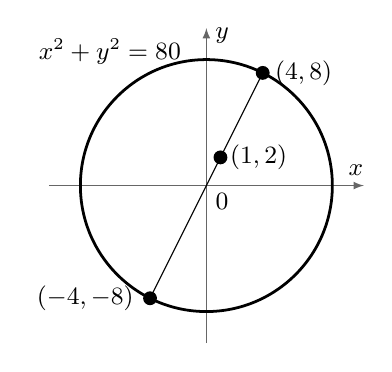
\begin{tikzpicture}
   \usetikzlibrary{arrows}
   \draw [black!60,line width=0.3pt,-latex] (-2,0) -- (2,0);
   \draw [black!60,line width=0.3pt,-latex] (0,-2) -- (0,2);
   \pgfputat{\pgfpointxyz{1.9}{0.2}{0}}{\pgfbox[center,center]{\small $x$}}
   \pgfputat{\pgfpointxyz{0.2}{1.9}{0}}{\pgfbox[center,center]{\small $y$}}
   \pgfputat{\pgfpointxyz{0.2}{-0.2}{0}}{\pgfbox[center,center]{\small $0$}}
   \draw [line width=1pt] (0,0) circle (1.6);
   \fill (0.7155,1.431) circle (2.5pt);
   \fill (0.1789,0.3578) circle (2.5pt);
   \fill (-0.7155,-1.431) circle (2.5pt);
   \draw (-0.7155,-1.431) -- (0.7155,1.431);
   \node [right] at (0.75,1.431) {\small $(4,8)$};
   \node [right] at (0.1789,0.3578) {\small $(1,2)$};
   \node [left] at (-0.8,-1.431) {\small $(-4,-8)$};
   \node [left] at (-0.2,1.7) {\small $x^2 + y^2 = 80$};
  \end{tikzpicture}}
 Substituting this into $g(x,y) = x^2 + y^2 = 80$ yields $5x^2=80$, so $x=\pm 4$. So the two constrained critical
 points are $(4,8)$ and $(-4,-8)$. Since $f(4,8)=45$ and $f(-4,-8)=125$, and since there must be points on the circle
 closest to and farthest from $(1,2)$, then it must be the case that $(4,8)$ is the point on the circle
 closest to $(1,2)$ and $(-4,-8)$ is the farthest from $(1,2)$ (see Figure 2.7.1).
 
 Notice that since the constraint equation $x^2 + y^2 = 80$ describes a circle, which is a bounded set in $\Real{2}$,
 then we were guaranteed that the constrained critical points we found were indeed the constrained maximum and
 minimum.
\end{exmp}
\hrule width \textwidth height 0.5pt
\medskip

The Lagrange multiplier method can be extended to functions of three variables.

\medskip
\hrule width \textwidth height 0.5pt
\begin{exmp}
 \begin{align*}
  \text{Maximize (and minimize)}&: ~ f(x,y,z) = x+z\\
  \text{given}&: ~ g(x,y,z) = x^2 + y^2 + z^2 = 1
 \end{align*}
 \par\noindent \emph{Solution:} Solve the equation $\nabla f(x,y,z) = \lambda \nabla g(x,y,z)$:
 \begin{align*}
  1 ~&=~ 2\lambda x\\
  0 ~&=~ 2\lambda y\\
  1 ~&=~ 2\lambda z
 \end{align*}
 The first equation implies $\lambda \ne 0$ (otherwise we would have $1=0$), so we can divide by $\lambda$ in the
 second equation to get $y=0$ and we can divide by $\lambda$ in the first and third equations to get
 $x=\frac{1}{2\lambda}=z$. Substituting these expressions into the constraint equation $g(x,y,z) = x^2 + y^2 + z^2 = 1$
 yields the constrained critical points $\biggl( \frac{1}{\sqrt{2}},0,\frac{1}{\sqrt{2}} \biggr)$ and
 $\biggl( \frac{-1}{\sqrt{2}},0,\frac{-1}{\sqrt{2}} \biggr)$. Since $f\biggl( \frac{1}{\sqrt{2}},0,\frac{1}{\sqrt{2}}
 \biggr) > f\biggl( \frac{-1}{\sqrt{2}},0,\frac{-1}{\sqrt{2}} \biggr)$, and since the constraint equation
 $x^2 + y^2 + z^2 = 1$ describes a sphere (which is bounded) in $\Real{3}$, then
 $\biggl( \frac{1}{\sqrt{2}},0,\frac{1}{\sqrt{2}} \biggr)$ is the constrained maximum point and
 $\biggl( \frac{-1}{\sqrt{2}},0,\frac{-1}{\sqrt{2}} \biggr)$ is the constrained minimum point.
\end{exmp}
\hrule width \textwidth height 0.5pt
\medskip

So far we have not attached any significance to the value of the Lagrange multiplier $\lambda$. 
We needed $\lambda$ only to find the constrained critical points, but made no use of its value. 
It turns out that $\lambda$ gives an approximation of the change in the value of the function $f(x,y)$ that we wish to maximize or minimize, when
the constant $c$ in the constraint equation $g(x,y)=c$ is changed by $1$.

For example, in Example \ref{exmp:rectlm} we showed that the constrained optimization problem
\begin{align*}
  \text{Maximize}&: ~ f(x,y) = xy\\
  \text{given}&: ~ g(x,y) = 2x + 2y = 20
\end{align*}
had the solution $(x,y) = (5,5)$, and that $\lambda = x/2 = y/2$. 
Thus, $\lambda = 2.5$. 
In a similar fashion we could
show that the constrained optimization problem
\begin{align*}
  \text{Maximize}&: ~ f(x,y) = xy\\
  \text{given}&: ~ g(x,y) = 2x + 2y = 21
\end{align*}
has the solution $(x,y) = (5.25,5.25)$. 
So we see that the value of $f(x,y)$ at the constrained maximum increased from
$f(5,5)=25$ to $f(5.25,5.25)=27.5625$, 
i.e. it increased by $2.5625$ when we increased the value of $c$ in the constraint equation $g(x,y)=c$ from $c=20$ to $c=21$. 
Notice that $\lambda = 2.5$ is close to $2.5625$, that is,
\begin{displaymath}
 \lambda ~\approx~ \Delta f ~=~ f(\text{new max. pt}) - f(\text{old max. pt}) ~.
\end{displaymath}


Note that
solving the equation $\nabla f(x,y) = \lambda \nabla g(x,y)$ means having to solve a system of two (possibly
nonlinear) equations in three unknowns, which as we have seen before, may not be possible to do. 
And the 3-variable case can get even more complicated. 
All of this somewhat restricts the usefulness of Lagrange's method to relatively simple functions. 
Luckily there are many numerical methods for solving constrained optimization problems, though we will not discuss them here.\footnote{See \cite{bss}.}

The following thereom is a vesion of Lagrange multiplier method for two constrains.
Note however that two constrains define a curve, 
so if parametrized the problem reduce to single-variable calculus.

\statethm{thm:lagrange}{
 {Let $f(x,y,z)$, $g_1(x,y,z)$ and $g_2(x,y,z)$ be smooth functions, and suppose that $c_1$ and $c_2$ are scalar constants such
 that $\nabla g_1(x,y,z)$ is not parallel to $\nabla g_2(x,y,z)$ for all $(x,y,z)$ that satisfy the equation $g_1(x,y,z) = c_1$ and $g_2(x,y,z) = c_2$. Then to solve the
 constrained optimization problem
 \begin{align*}
  \text{Maximize (or minimize)}:& ~ f(x,y,z)\\
  \text{given}:& ~ g_1(x,y,z) = c_1 ~,
              \\&~g_2(x,y,z) = c_2 ~
 \end{align*}
 find the points $(x,y,z)$ that solve the equation 
 \[\nabla f(x,y,z) = \lambda \nabla g_1(x,y,z)+\mu \nabla g_2(x,y,z)\] 
 for some constants
 $\lambda$ and $\mu$. 
 If there is a constrained maximum or
 minimum, then it must be such a point.}
}



\startexercises\label{sec2dot7}
\probs{A}
\begin{enumerate}[\bfseries 1.]
 \item Find the constrained maxima and minima of $f(x,y) = 2x+y$ given that $x^2 + y^2 =4$.
 \item Find the constrained maxima and minima of $f(x,y) = xy$ given that $x^2 + 3y^2 =6$.
 \item Find the points on the circle $x^2 + y^2 = 100$ which are closest to and farthest from the point $(2,3)$.
\suspend{enumerate}
\probs{B}
\resume{enumerate}[{[\bfseries 1.]}]
 \item Find the constrained maxima and minima of $f(x,y,z) = x+y^2 +2z$ given that $4x^2 + 9y^2 -36z^2 =36$.
 \item Find the volume of the largest rectangular parallelepiped with edges parallel to the coordinate axis that can be inscribed in the ellipsoid
  \begin{displaymath}
   \frac{x^2}{a^2} + \frac{y^2}{b^2} + \frac{z^2}{c^2} = 1 ~.
  \end{displaymath}
\end{enumerate}
